\section{Performance and Analysis}
In this chapter we present the results obtained by these two algorithm. We use 13 dataset to test the algorithm, and we analyze the performance globally on the entire algorithm but also locally on specific phases and sub-phases in order to highlight the point of strengths and the weakness of both the algorithm. In this chapter we firstly present the datasets on which we have executed our test. Then we give an overlook on the results obtained that are useful for the subsequent analysis which, in turn, we dived in two parts: in the first part we analyze the contribution of the pruning approach on each algorithm; in the second part we make a comparison between the two algorithms, in order to enhance when one algorithm performs better than the other. This consideration are on base to the adaptive algorithm that we present in the next chapter. It implements the logic of the two algorithm and select to use the best basing on the situation, so the information that we have collect in this part are foundamental for the design choice that we make. 
\subsection{Datasets}\label{Dataset}
In this section we present the 13 dataset used in this thesis. These datasets coming from three main sources: the Stanford Stanford Large Network Dataset Collection (also known as SNAP) \cite{snap}, the Florida Sparse Matrix Collection \cite{florida-matrix} and the the Koblenz Network Collection (also known as KONECT)  \cite{konect}. In the Table \ref{tab:dataset} there are a briefly presentation of the dataset and in Figure \ref{fig:dataset-degree-distribution} there are the degree distribution of the graphs.  We point out that even if all this graph are unweighted, some of it are directed: during the parsing phase we doesn't keep the "directness" of the graph, and we treat it as a undirected one as required from the algorithm. In addition, if in the original graph there are some repeated edges, we consider it once. In the table \ref{tab:dataset} the number of edges are those obtained after this parsing, ordered by increasing edges number. Now we present the datasets:
\begin{table}
	\centering
	\begin{tabular}{ |l||c||r|r|}
		\hline
		\multicolumn{4}{|c|}{Datasets} \\
		\hline
		Name& Source &  Number of nodes  & Number of edges\\
		\hline
		coPapersDBLP & Florida  & 540 486    & 15 245 729\\
		patentCite & KONECT &3 774 768 & 16 518 947 \\
		packing-500x100x100-b050 & Florida & 2 145 839 & 17 488 243 \\
		soc-pokec-relationship & SNAP &1 632 803 & 22 301 964 \\ 
		delaunay\_n23 & Florida &8 388 608 & 25 165 784\\
		soc-LiveJournal1 & SNAP & 4 847 571 & 43 369 619 \\
		wikipedia\_link\_ja & KONECT & 1 610 638 & 56 237 763\\
		hollywood-2009 & Florida &1 139 905 & 57 515 616 \\
		wikipedia\_link\_it & KONECT & 1 865 965 & 68 049 979\\
		wikipedia\_link\_fr & KONECT & 3 023 165 & 83 472 152\\
		com-orkut & SNAP &3 072 441 &117 185 083\\
		wikipedia\_en(dbpedia) & KONECT & 18 268 991 & 126 890 209 \\
		indochina-2004 & Florida & 7 414 768 & 153 487 303 \\
		\hline
	\end{tabular}
	\caption{\label{tab:dataset}Datasets overview}
\end{table} 
\begin{itemize}
	\item \textbf{coPapersDBLP:} this graph model the citation and co-author network from the DBLP - Digital Bibliography and Library Project. Each node represent an author and each edge a citation.
	\item \textbf{patentCite:} This is the citation network of patents registered with the United States Patent and Trademark Office. Each node is a patent, and a directed edge represents a patent and an edge represents a citation. The network contain loops. This graph is also directed.
	\item \textbf{packing-500x100x100-b050:} this is a synthetic graph from numerical simulation.  
	\item \textbf{soc-pokec:} Pokec is the most popular on-line social network in Slovakia. Pokec has been provided for more than 10 years and connects more than 1.6 million people. This dataset map the relationship between people.
	\item \textbf{delaunay\_n23:} given a random set of point, in this graph represent a Delaunay triangulations of them.
	\item \textbf{soc-LiveJournal1}: LiveJournal is a free on-line community with almost 10 million members; a significant fraction of these members are highly active. LiveJournal allows members to maintain journals, individual and group blogs, and it allows people to declare which other members are their friends they belong. This graph model these friendship relations. 
	\item \textbf{wikipedia\_link\_jp:} This network consists of the wikilinks of the Wikipedia in the Japanese language (.ja). Nodes are Wikipedia articles, and directed edges are hyperlinks. Only pages in the article namespace are included. This graph is directed and some self-loop is possible.
	\item \textbf{hollywood-2009}: The graph of           
	movie actors. Vertices are actors, and two actors are joined             
	by an edge whenever they appeared in a movie together. The data date back to 2009. 
	\item \textbf{wikipedia\_link\_it:} This network consists of the wikilinks of the Wikipedia in the Italian language (it). Nodes are Wikipedia articles, and directed edges are hyperlinks. Only pages in the article namespace are included. This graph is directed and some self-loop is possible.
	\item \textbf{wikipedia\_link\_fr:} This network consists of the wikilinks of the Wikipedia in the French language (.fr). Nodes are Wikipedia articles, and directed edges are hyperlinks. Only pages in the article namespace are included. This graph is directed and some self-loop is possible.
	\item \textbf{com-orkut:} Orkut is a social-network where users form friendship each other: the nodes represent the users and the edges the friendship between them.
	\item \textbf{wikipedia\_en (dbpedia)}: The network is the hyperlink network of Wikipedia, as extracted in DBpedia. Nodes are pages in Wikipedia and edges correspond to hyperlinks (also known as wikilinks). The edges correspond to the relationships in DBpedia.
	Network info. The original graph is directed and multiple edges are possible.
	\item \textbf{indochina-2004}: A fairly large crawl of the country domains of Indochina performed for the Nagaoka University of Technology. This is a directed graph and each node represent a site and each edge a link from one site to another.
\end{itemize}

\begin{figure}
	\centering
	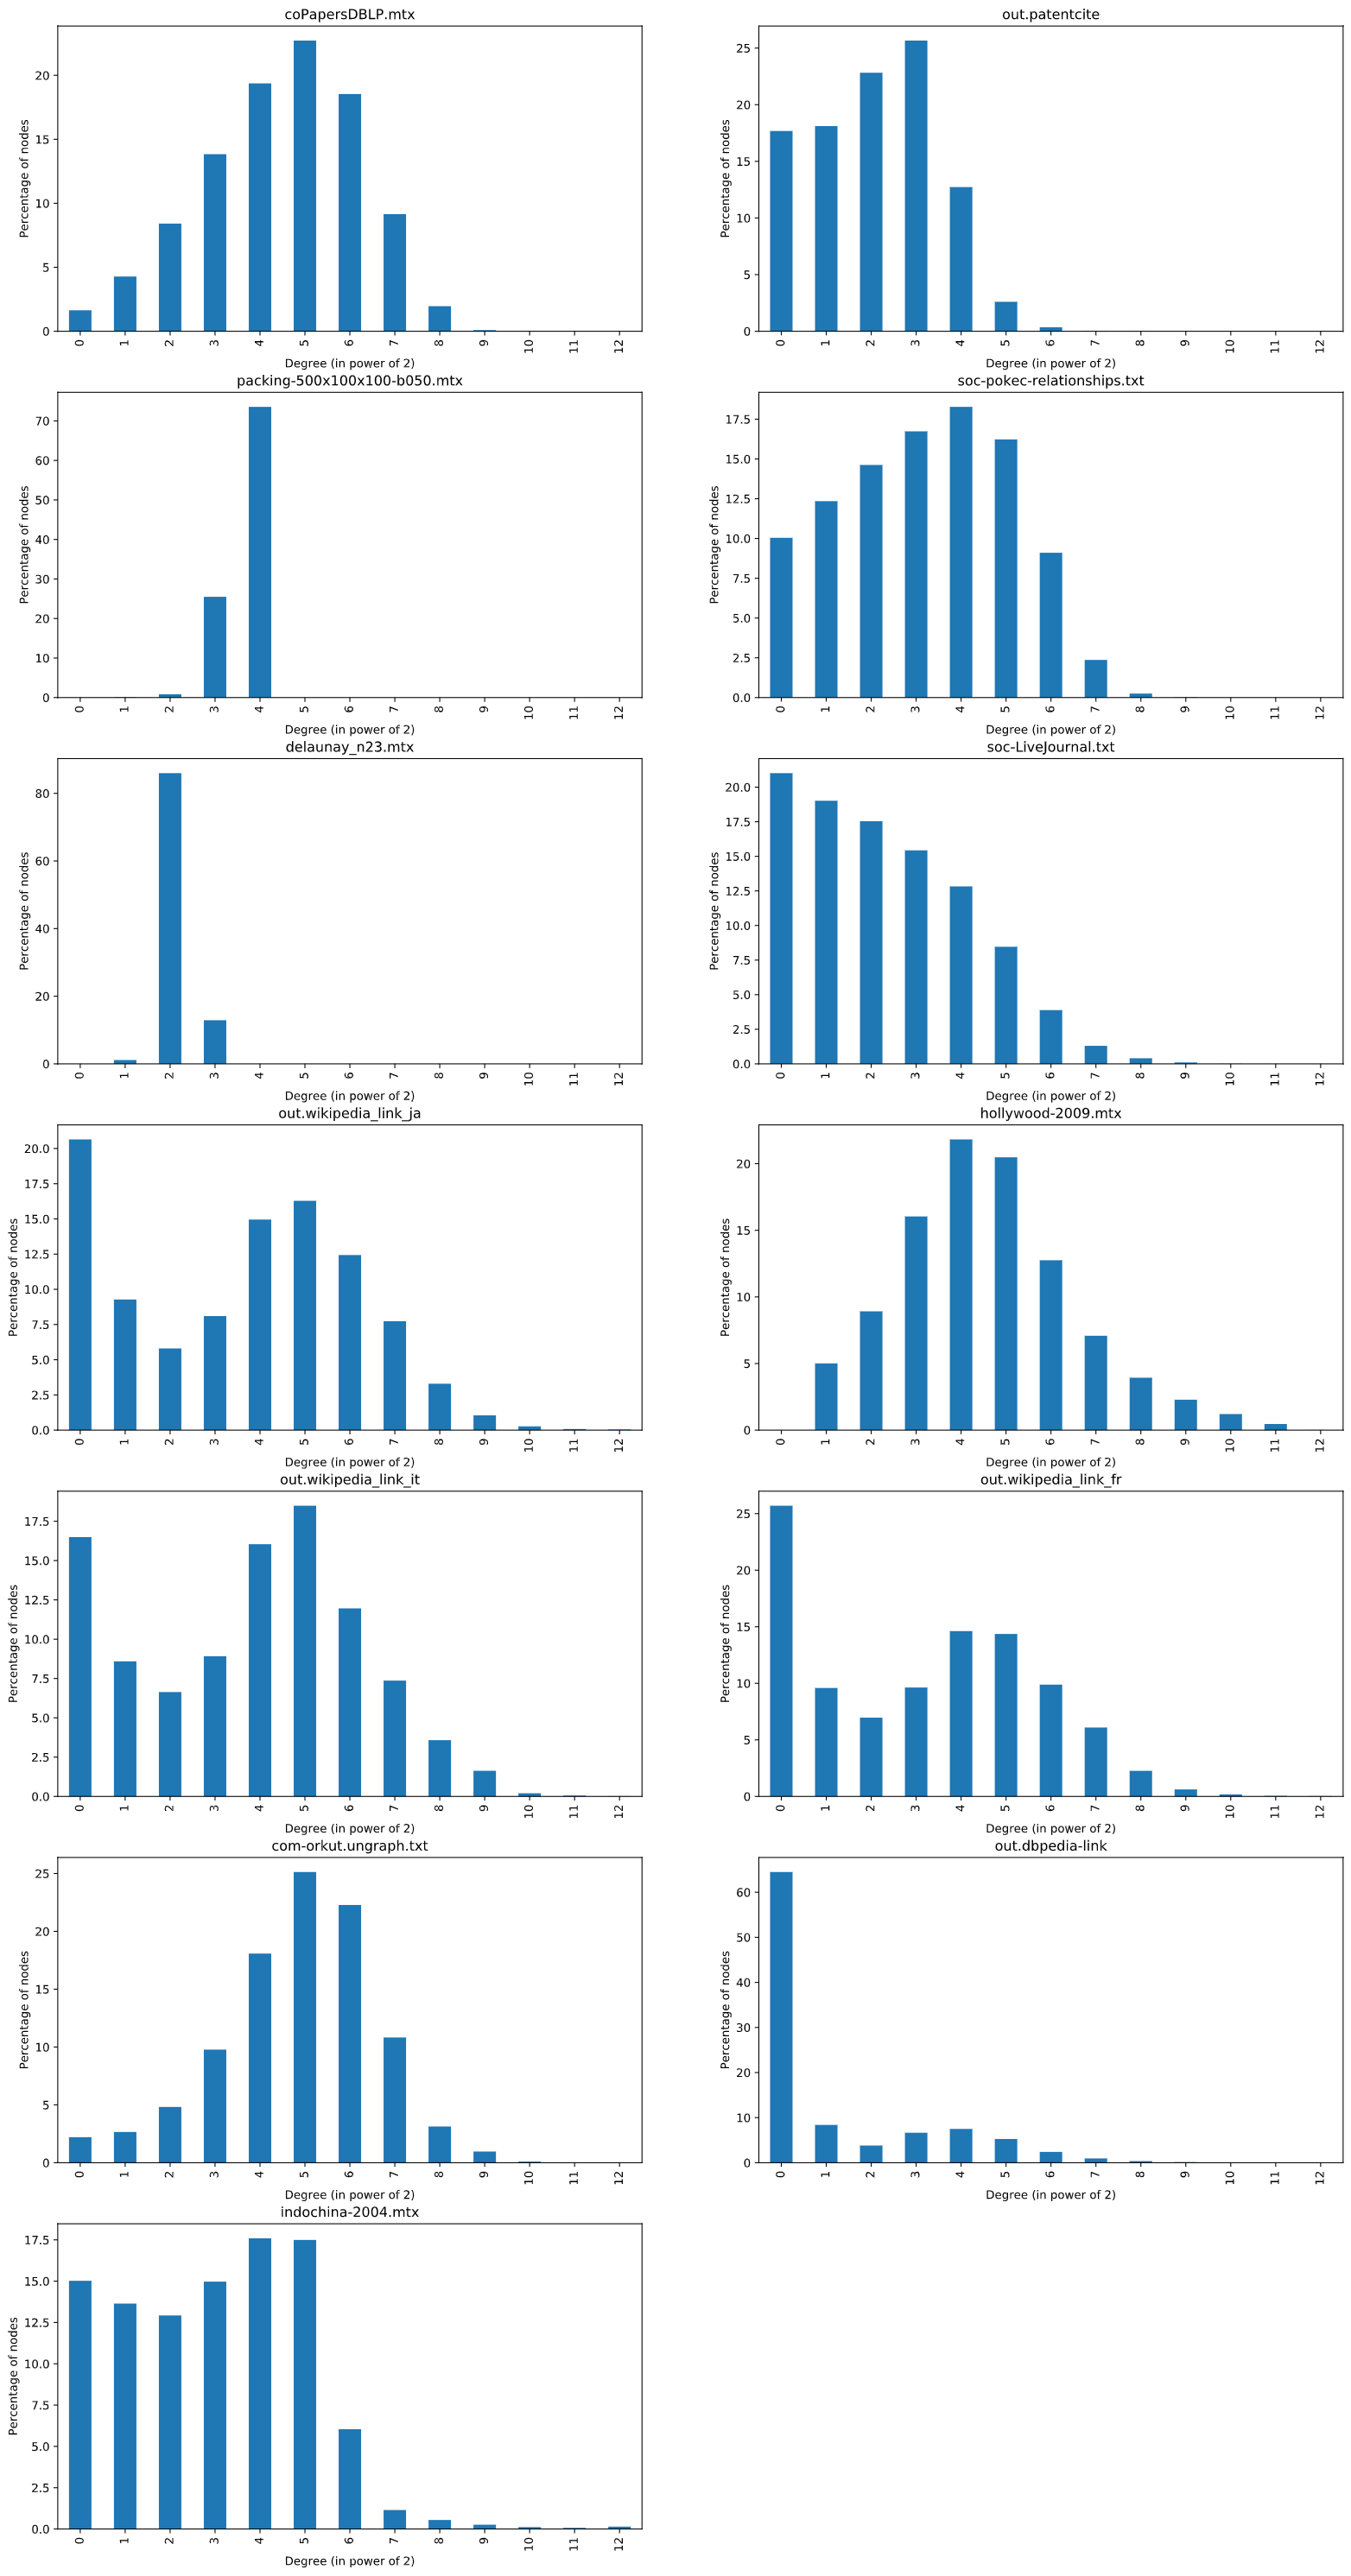
\includegraphics[width=1\linewidth]{0-resources/dataset-degree-distribution.png}
	\caption{Degree distribution in the datasets: we divide the nodes in ordered classes where in the class $i$ there are all the nodes with degree in range $[2^i, 2^{i+1})$. On the $x$-axes there are these classes; on the $y$ axes there is the percentage of nodes assigned to them.}
	\label{fig:dataset-degree-distribution}
\end{figure}
\newpage
\subsection{Results Overview}
In this section we present an overview of the obtained results and we make some general consideration about it. Some more insights about the first optimization phase and about the aggregation phase are presented next and we make some consideration in light of what we present in this section.\\ 
The algorithms was run on a Ubuntu 18.04.4 LTS machine with a 2.10GHz  Intel(R) Xeon(R) Silver 4110 CPU, a TITAN Xp GPU with 12 GB of memory and CUDA 10.2. To run our code we need a Nvidia GPU with a compute capability $\geq$ 3.5 due to the 64 bits \verb|atomicMax| operation used in PH-Louvain. This GPU have a compute capability 6.1, so it comply with the technical specification.
We remark that we keep executing our optimization phase until the value of $\Delta Q$ between the various iteration is greater than a threshold $t$. Both our parallel version in the test uses $t = 0.01$.\\
\begin{table}[h]
	\centering
	\begin{tabular}{ |l||r||r|r|}
		\hline
		\multicolumn{4}{|c|}{Modularity Score} \\
		\hline
		Graph & Sequential & PSR-Louvain & PH-Louvain \\
		\hline
		coPapersDBLP 			& 0.8490 & 0.8544 & 0.8544 \\
		patentCite 				& 0.8095 & 0.7911 & 0.7878 \\
		packing-500x100x100-b050& 0.9353 & 0.9434 & 0.9416 \\
		soc-pokec-relationship	& 0.6837 & 0.6934 & 0.6852 \\ 
		delaunay\_n23 			& 0.9881 & 0.9856 & 0.9857 \\
		soc-LiveJournal1 		& 0.7251 & 0.7491 & 0.7482 \\
		wikipedia\_link\_ja 	& 0.5928 & 0.5690 & 0.5724 \\
		hollywood-2009 			& 0.7511 & 0.7542 & 0.7542 \\
		wikipedia\_link\_it 	& 0.7221 & 0.7190 & 0.7196 \\
		wikipedia\_link\_fr 	& 0.6777 & 0.6834 & 0.6871 \\
		com-orkut 				& 0.6545 & 0.6613 & 0.6629 \\
		wikipedia\_en(dbpedia) 	& 0.6629 & 0.6612 & 0.6618 \\
		indochina-2004 			& 0.9638 & 0.9632 & 0.9632 \\
		\hline
	\end{tabular}
	\caption{\label{tab:mod}Modularity result}
\end{table} \\
First of all, we analyze the modularity score obtained by the two algorithms respect to the sequential version as presented in \cite{Blondel_2008} to check the correctness of the our algorithm. In the Table \ref{tab:mod} are exposed the obtained results. We notice that both the score of the algorithm are in pair between them and also with the sequential version for all the graphs, and in some case we obtain also a better result in the parallel implementations respect to the sequential version. This  may be due to the parallel optimization, changing all the communities assigned to the vertices simultaneously, can avoid some local maxima.
\begin{table}
	\centering
	\begin{tabular}{ |l||r||r|r|}
		\hline
		\multicolumn{4}{|c|}{Execution Times} \\
		\hline
		Graph & Sequential & PSR-Louvain & PH-Louvain \\
		\hline
		coPapersDBLP 			&  11 906.89 &   419.59 &  412.79 \\
		patentCite 				&  88 620.13 & 1 796.88 & 2 555.14 \\
		packing-500x100x100-b050&  13 746.14 & 1 045.25 & 1 090.03 \\
		soc-pokec-relationship	&  30 162.70 & 1 843.95 & 2 186.81 \\ 
		delaunay\_n23 			&  44 392.42 & 1 020.23 & 1 319.22 \\
		soc-LiveJournal1 		&  77 225.64 & 2 187.45 & 2 677.51 \\
		wikipedia\_link\_ja 	&  76 816.01 & 2 654.88 & 2 305.11 \\
		hollywood-2009 			&  52 306.71 & 2 092.09 & 1 758.27 \\
		wikipedia\_link\_it 	&  82 599.92 & 3 875.04 & 2 732.99 \\
		wikipedia\_link\_fr 	& 115 977.81 & 3 910.95 & 3 273.91 \\
		com-orkut 				& 193 835.34 & 7 566.90 & 7 484.10 \\
		wikipedia\_en(dbpedia) 	& 300 431.38 & 5 287.65 & 6 464.03 \\
		indochina-2004 			& 113 195.87 & 2 899.50 & 2 303.52 \\
		\hline
	\end{tabular}
	\caption{\label{tab:execution_time}Execution Time in milliseconds}
\end{table} \\
In the Table \ref{tab:execution_time} there are the execution time of the two algorithms respect to the sequential version. We notice a big improvement in the performance for both the algorithm respect to the sequential version: we obtain a speed-up in range of a variable factor from 12 to 56 for our two algorithms. 
Besides, we notice that, according to the graph analyzed, the two algorithms obtain different performance. In some case one approach outperforms the other of even more than one second. In the following sections we analyze in details this two algorithm to discover the motivation of this different performances.  
\subsection{Pruning analysis}
In this section, we analyze the effectiveness of the pruning approach: we focus our research on the first optimization phase. As we said previously, the first optimization phase is the most time-requiring phase, consuming about 80\% of the time \cite{wickramaarachchi2014fast}, so the pruning approach should increase the performance especially in this phase. For this reason, we concentrate our analysis of this technique over it.
\begin{figure}[h]
	\centering
	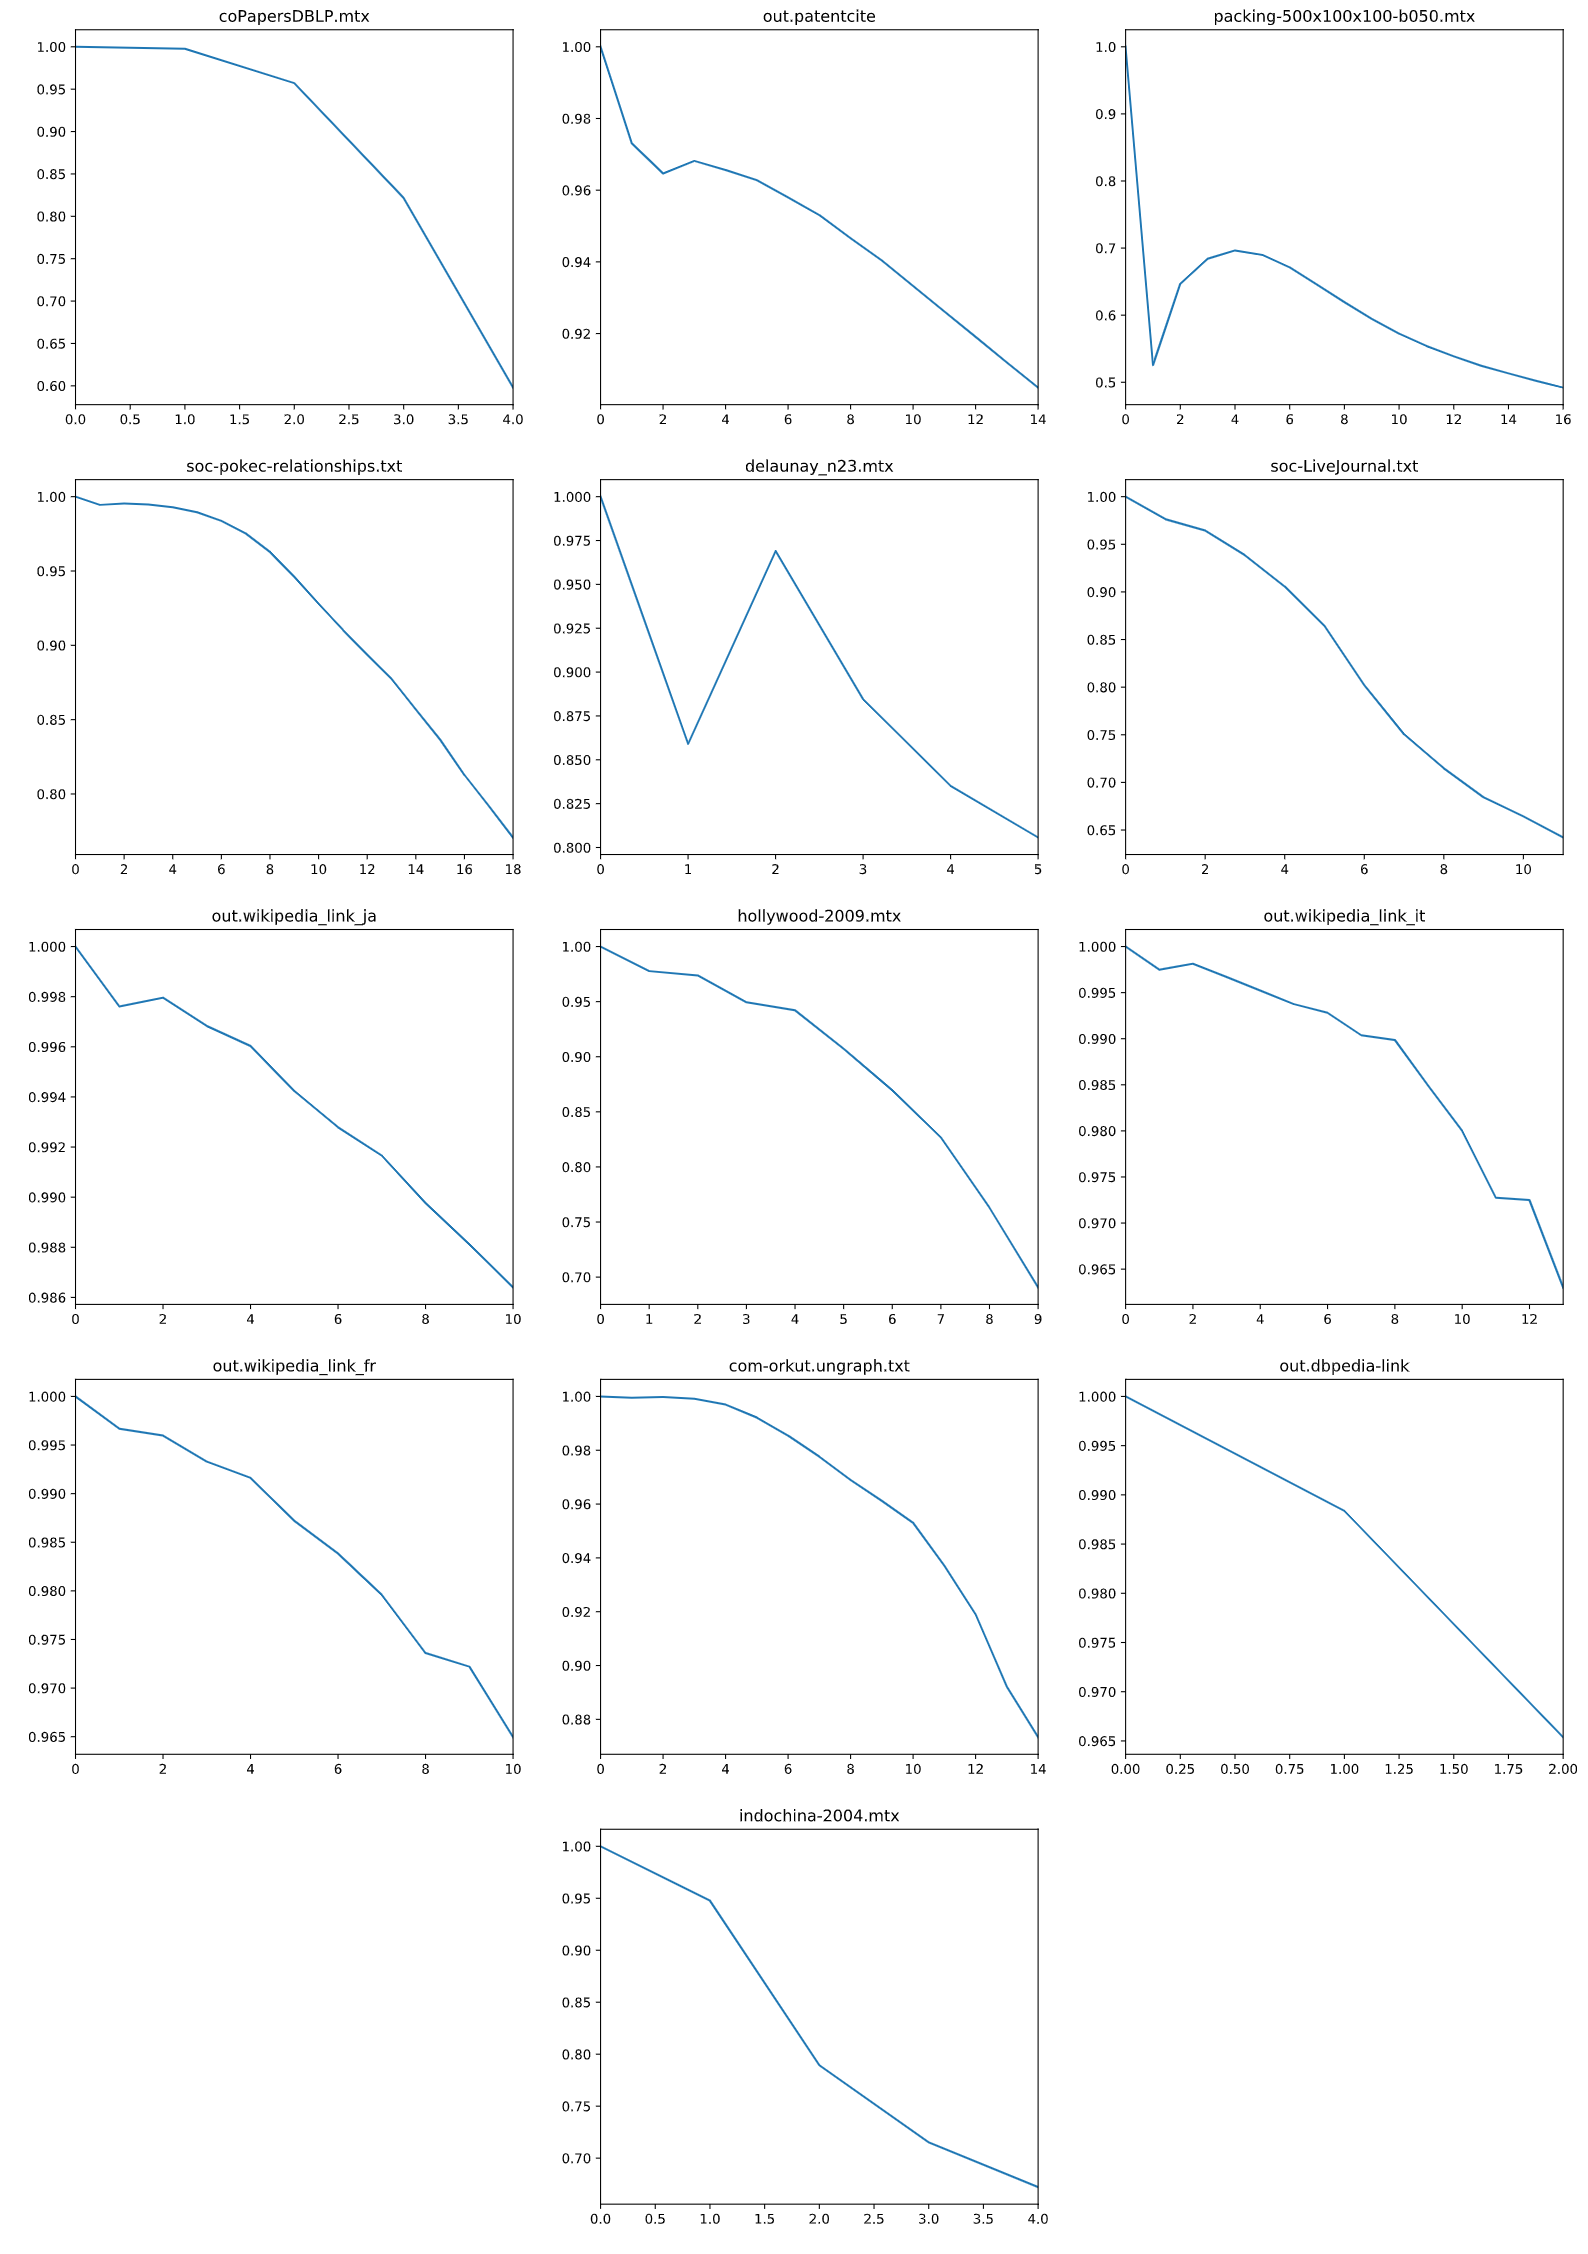
\includegraphics[width=1\linewidth]{0-resources/edge-percentage}
	\caption{Percentage of edge analyzed in the first optimization phase.}
	\label{fig:edge-percentage}
\end{figure}
First of all we present the percentage of the edges that we analyze in each iteration of the optimization phase (Figure \ref{fig:edge-percentage}). The number of the edges analyze are quite similar for both the algorithms. Exluding certain fluctuation at the earliest stage (we remark also that the two graph with the highest noise are two syntetic ones, i.e. packing-500x100x100-b050 and delaunay\_n23), we notice that the portion of the edges analyzed tend to decrease iteration by iteration. The percentage of reduction highly depends on the graph exterminated: we have the smallest reduction for the wikipedia\_link\_ja (only the $\sim\%2$ of the total are excluded in the last iteration); instead, in the graph packing-500x100x100-b050, we have run the optimization only on the $\sim\%50$ of the edges of the graph in last iteration. Our study on the dataset doesn't find any direct correlation between the decrease of the number of the edges analyzed and the degree distribution of the nodes presented in Figure \ref{fig:dataset-degree-distribution}.
\subsubsection{PSR-Louvain analysis}
\begin{figure}[h]
	\centering
	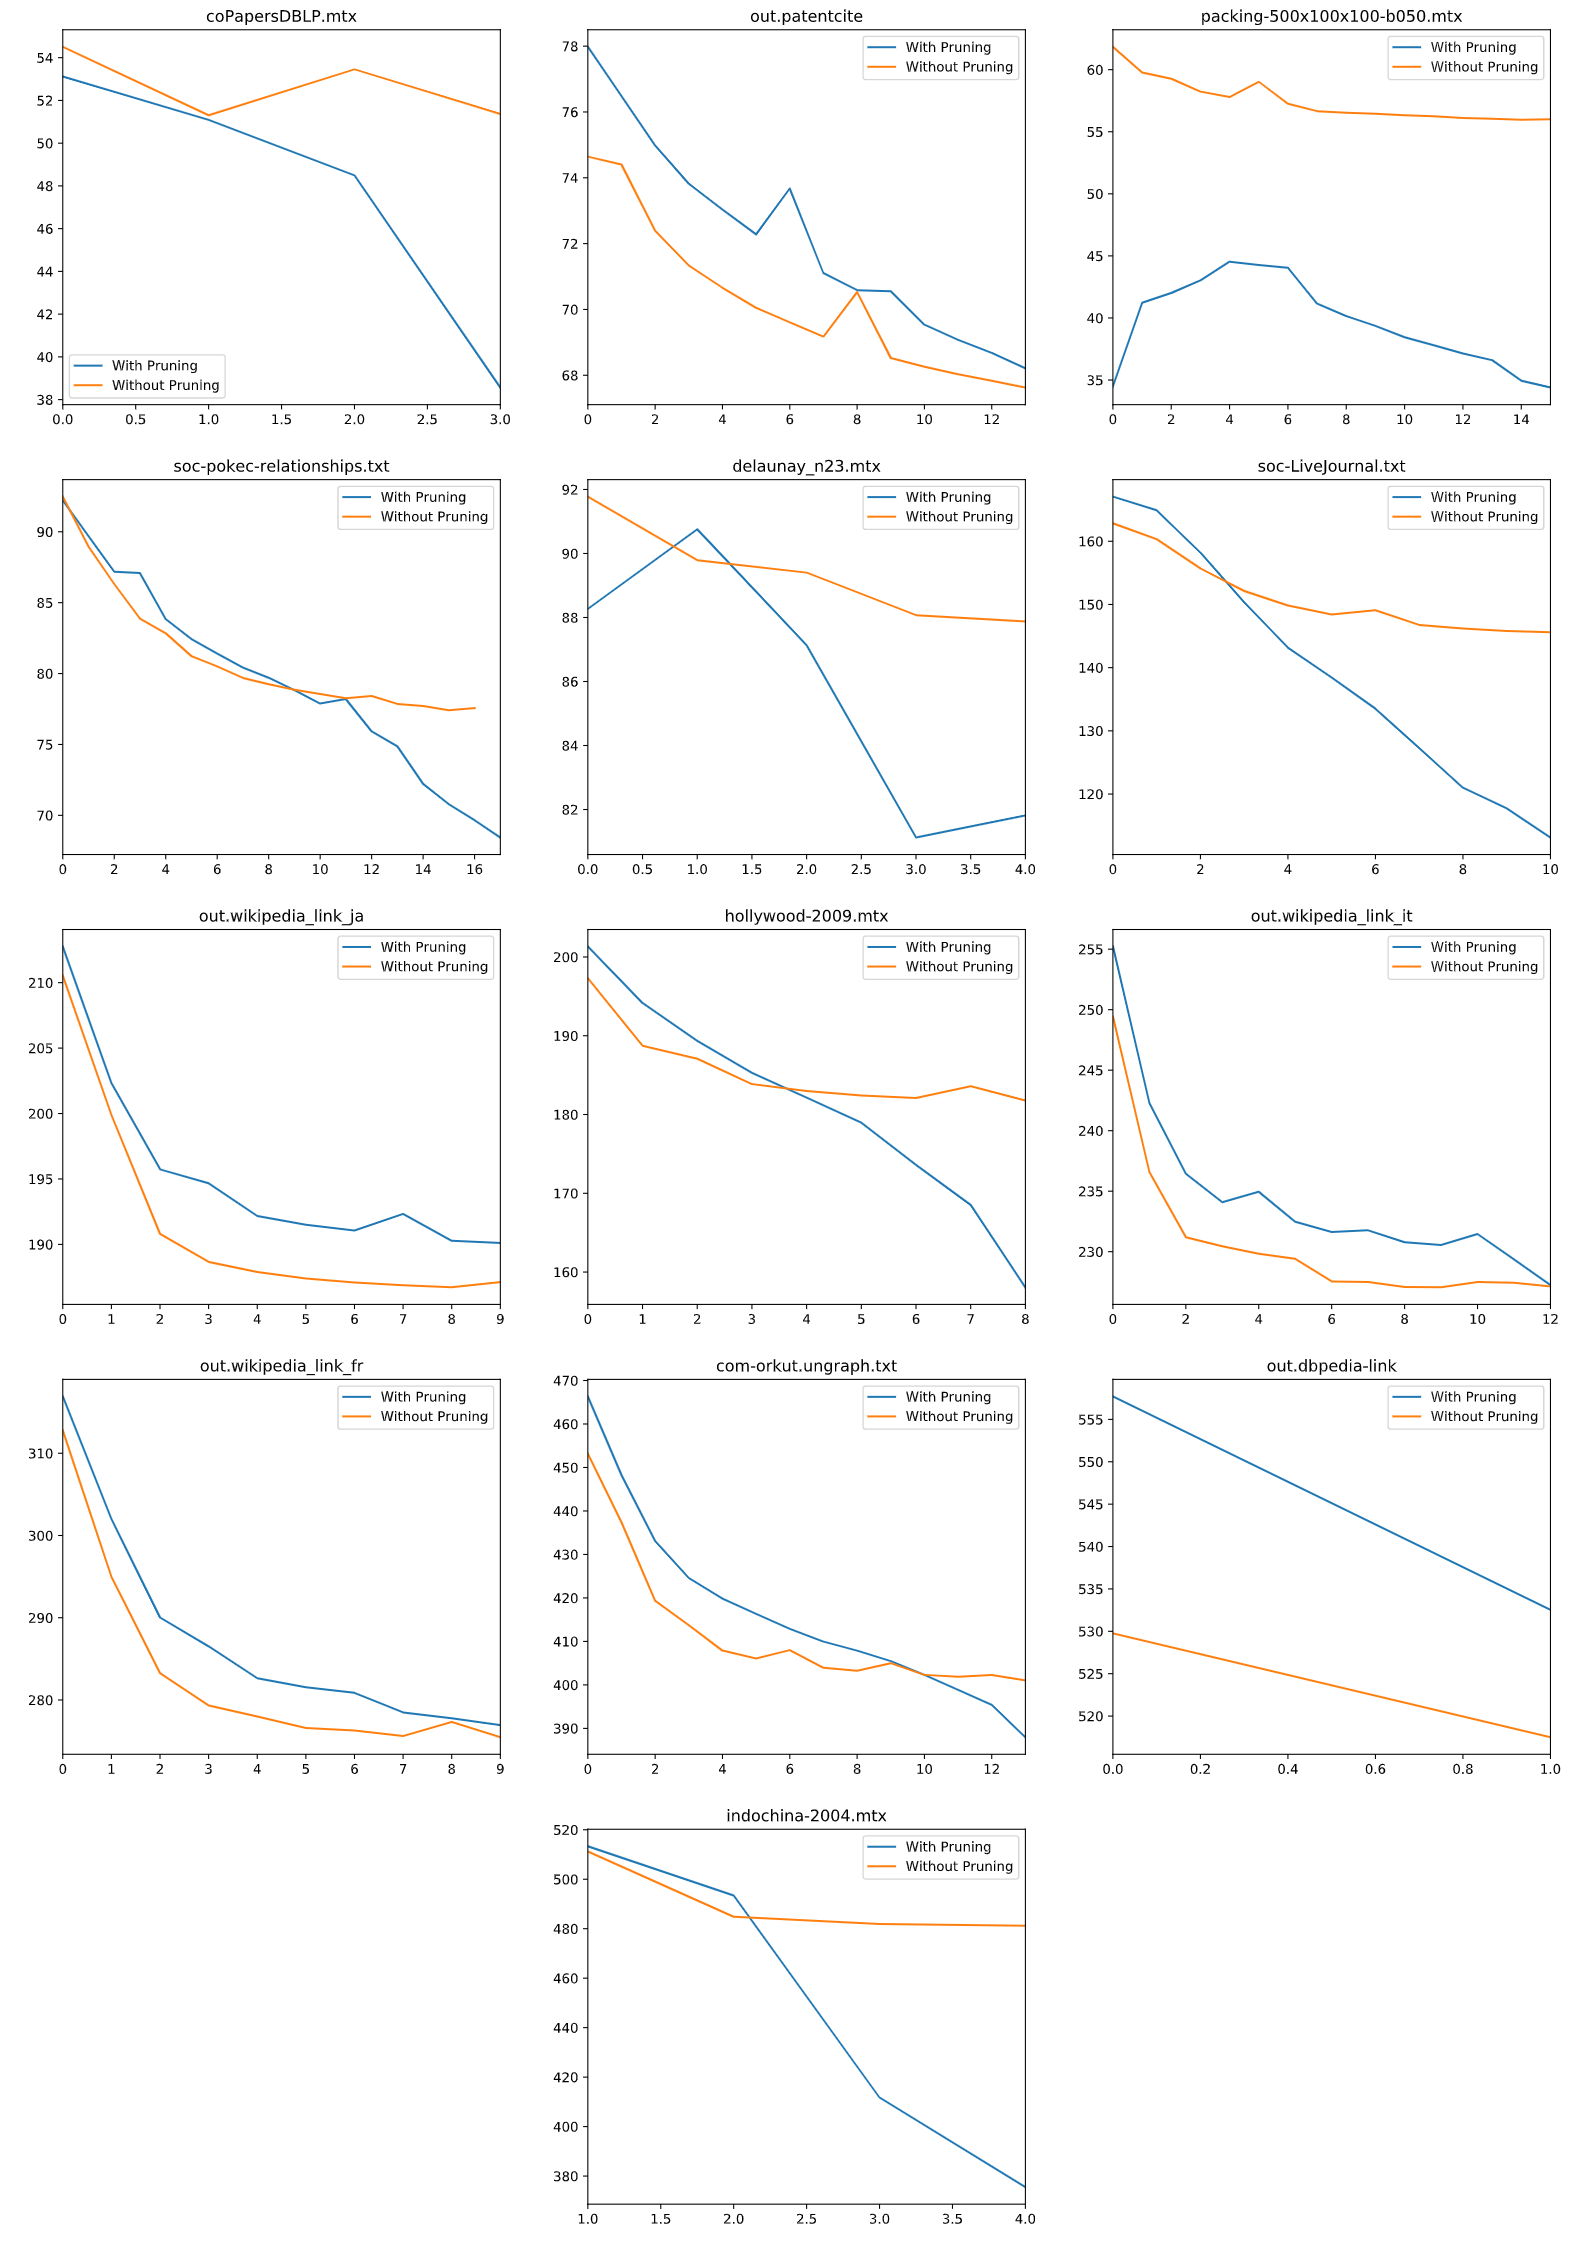
\includegraphics[width=1\linewidth]{0-resources/sort-prune-vs-no-prune}
	\caption{Comparison of the execution time between the Prune-Sort-Reduce (in blue) and a version of comparison without the Pruning approach (in orange) for each execution of the first optimization phase, excluding the first one.}
	\label{fig:prun-vs-no}
\end{figure}
\noindent Now we evaluate the impact in terms of time of the pruning approach in the PSR-Louvain algorithm: to do this, we create a comparison version of the algorithm from the presented one. This version doesn't prune the node in the Copy sub-phase and doesn't collect the data used to create the support pruning array in the last two sub-phases (the first one only update the community assign to each node; the second one is skipped). The execution times of each iteration of the first phase are illustrated in the Figure \ref{fig:prun-vs-no}. We exclude from this graphic the first iteration because this one doesn't make the same step of the other due to its special optimization (Chapter \ref{f-1}). We notice that the reduction in terms of times in the pruning version is proportional to the reduction of edges analyzed: in the graph in which the reduction of the edges analyzed highly decrease, the pruning version outperform the the standard version; in the graph in which the reduction in terms of edges are small, the execution times are quite similar: the pruning algorithm is slower up to $\sim15$ ms at iteration (in dbpedia-link) due to the fact that the computation of the pruning information requires some extra time but the reduction that leads to is smaller. In general we see that the ratio between execution times of the pruning version and the non-pruning one is in pair with the number of nodes pruned in each iteration. We notice also that the execution times decrease iteration by iteration even for the version without the pruning: this is caused by the reduction in terms of the time of the update subphase, as we can see in the \ref{fig:livejournal-comparison} is illustrated the contribution of each sub-phase in terms of time to for each iteration for the pruning version and the standard in the LiveJournal1 dataset.
\begin{figure}
	\centering
	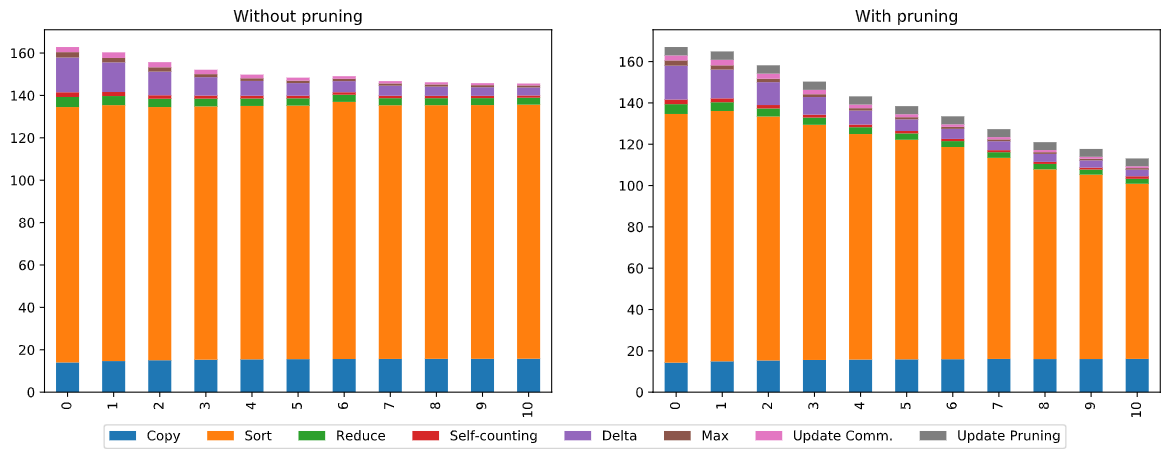
\includegraphics[width=1\linewidth]{0-resources/livejournal-comparison-sort.png}
	\caption{Comparison of the execution time between the Prune-Sort-Reduce (on the left) and a version of comparison without the Pruning approach (on the pruning) for each execution of the first iteration phase in the LiveJournal1 dataset. We highlight the contribution of each sub-phase in terms of time.}
	\label{fig:livejournal-comparison}
\end{figure}
We notice that the Sort sub-phase is the most consuming one and this behaviour is similar also in the other graph: this sub-phase at least 50\% of the time, reaching peek of even more than 80\% of the time in the first and in the last graph (Figure \ref{fig:suphases-sort}). From the Figure \ref{fig:livejournal-comparison}, we notice also that the pruning on the data in input have a direct effect on the sorting phase and the decreasing in terms of time is proportional to the number of the edges pruned (as we can see by comparing Figure \ref{fig:suphases-sort} and Figure \ref{fig:edge-percentage}). The pruning update has a small impact to the total execution time. 
\begin{figure}[t!]
	\centering
	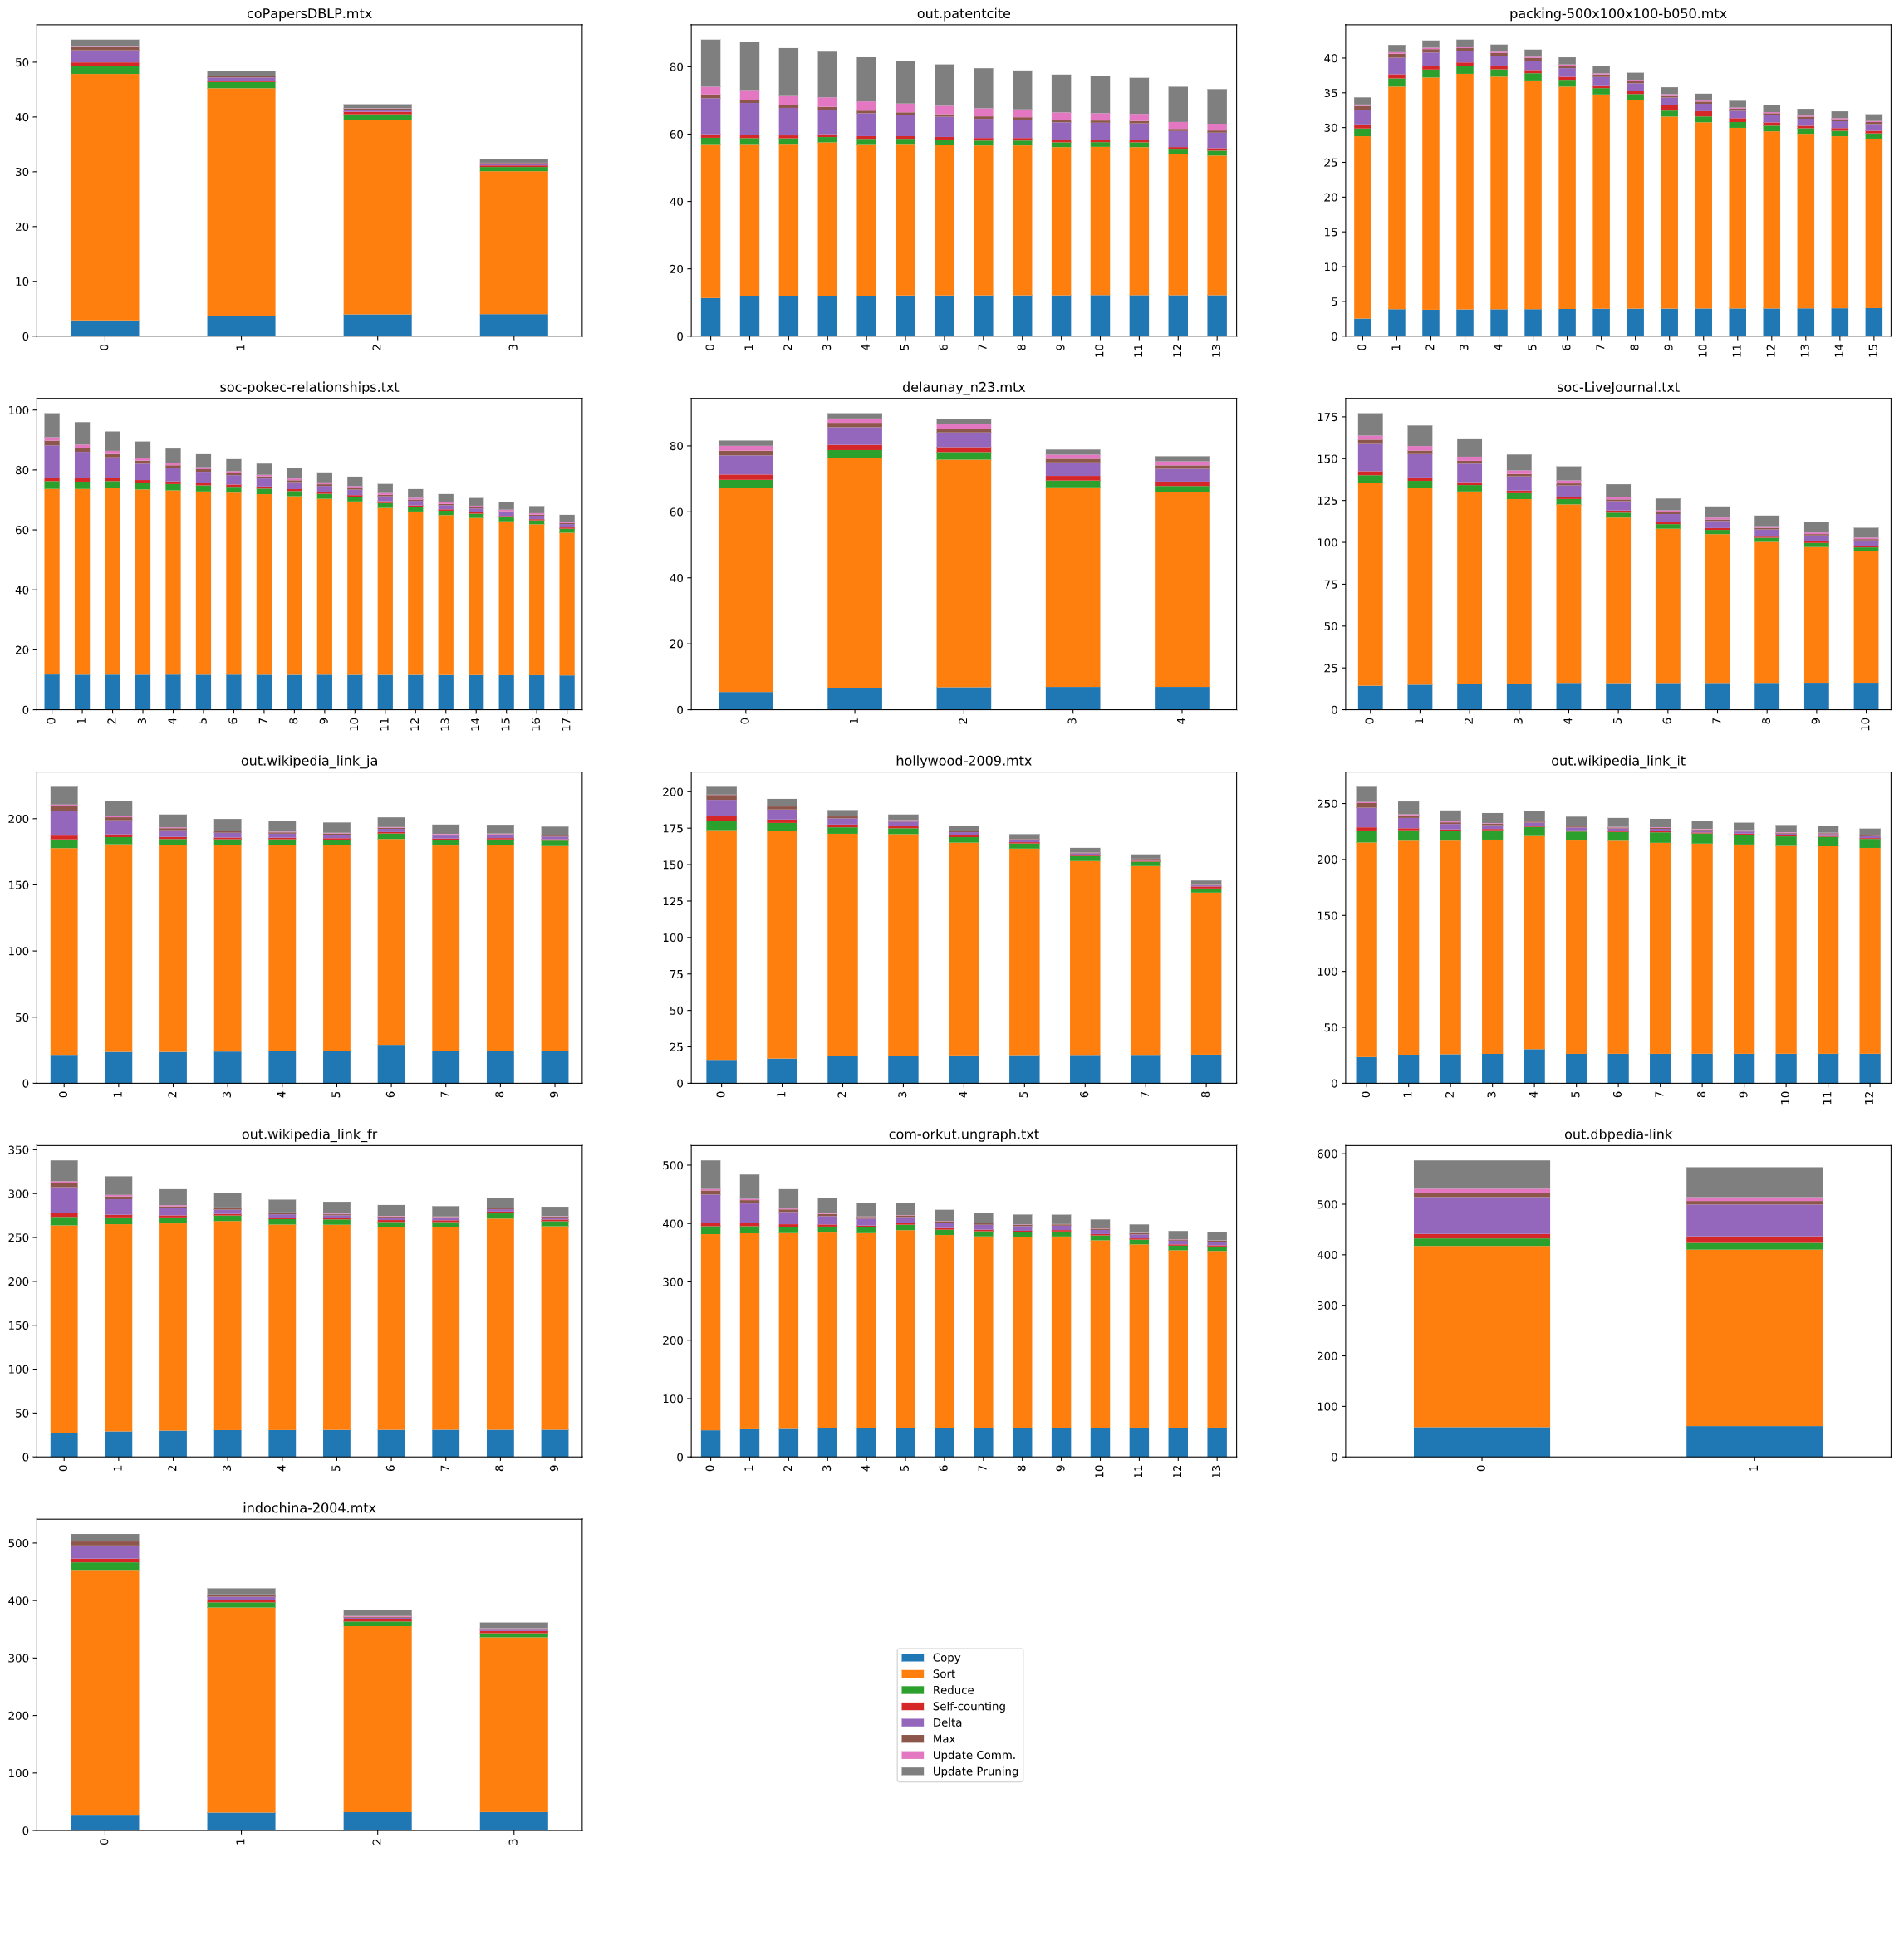
\includegraphics[width=1\linewidth]{0-resources/suphases-sort}
	\caption{Contribution of each sub-phase in terms of time for each iteration of the first optimization phase. }
	\label{fig:suphases-sort}
\end{figure}
In conclusion, even if the pruning approach isn't always effective and can introduce a little overhead, the gain in terms of time that we obtain when we prune a portion of the edges are high, therefore adding the pruning approach is a valid optimization techniques for the algorithm that use a sort-reduce pattern to aggregate. 
\subsubsection{Hashmap algorithm analysis}\label{hashmap-analysis}
\begin{figure}[h]
	\centering
	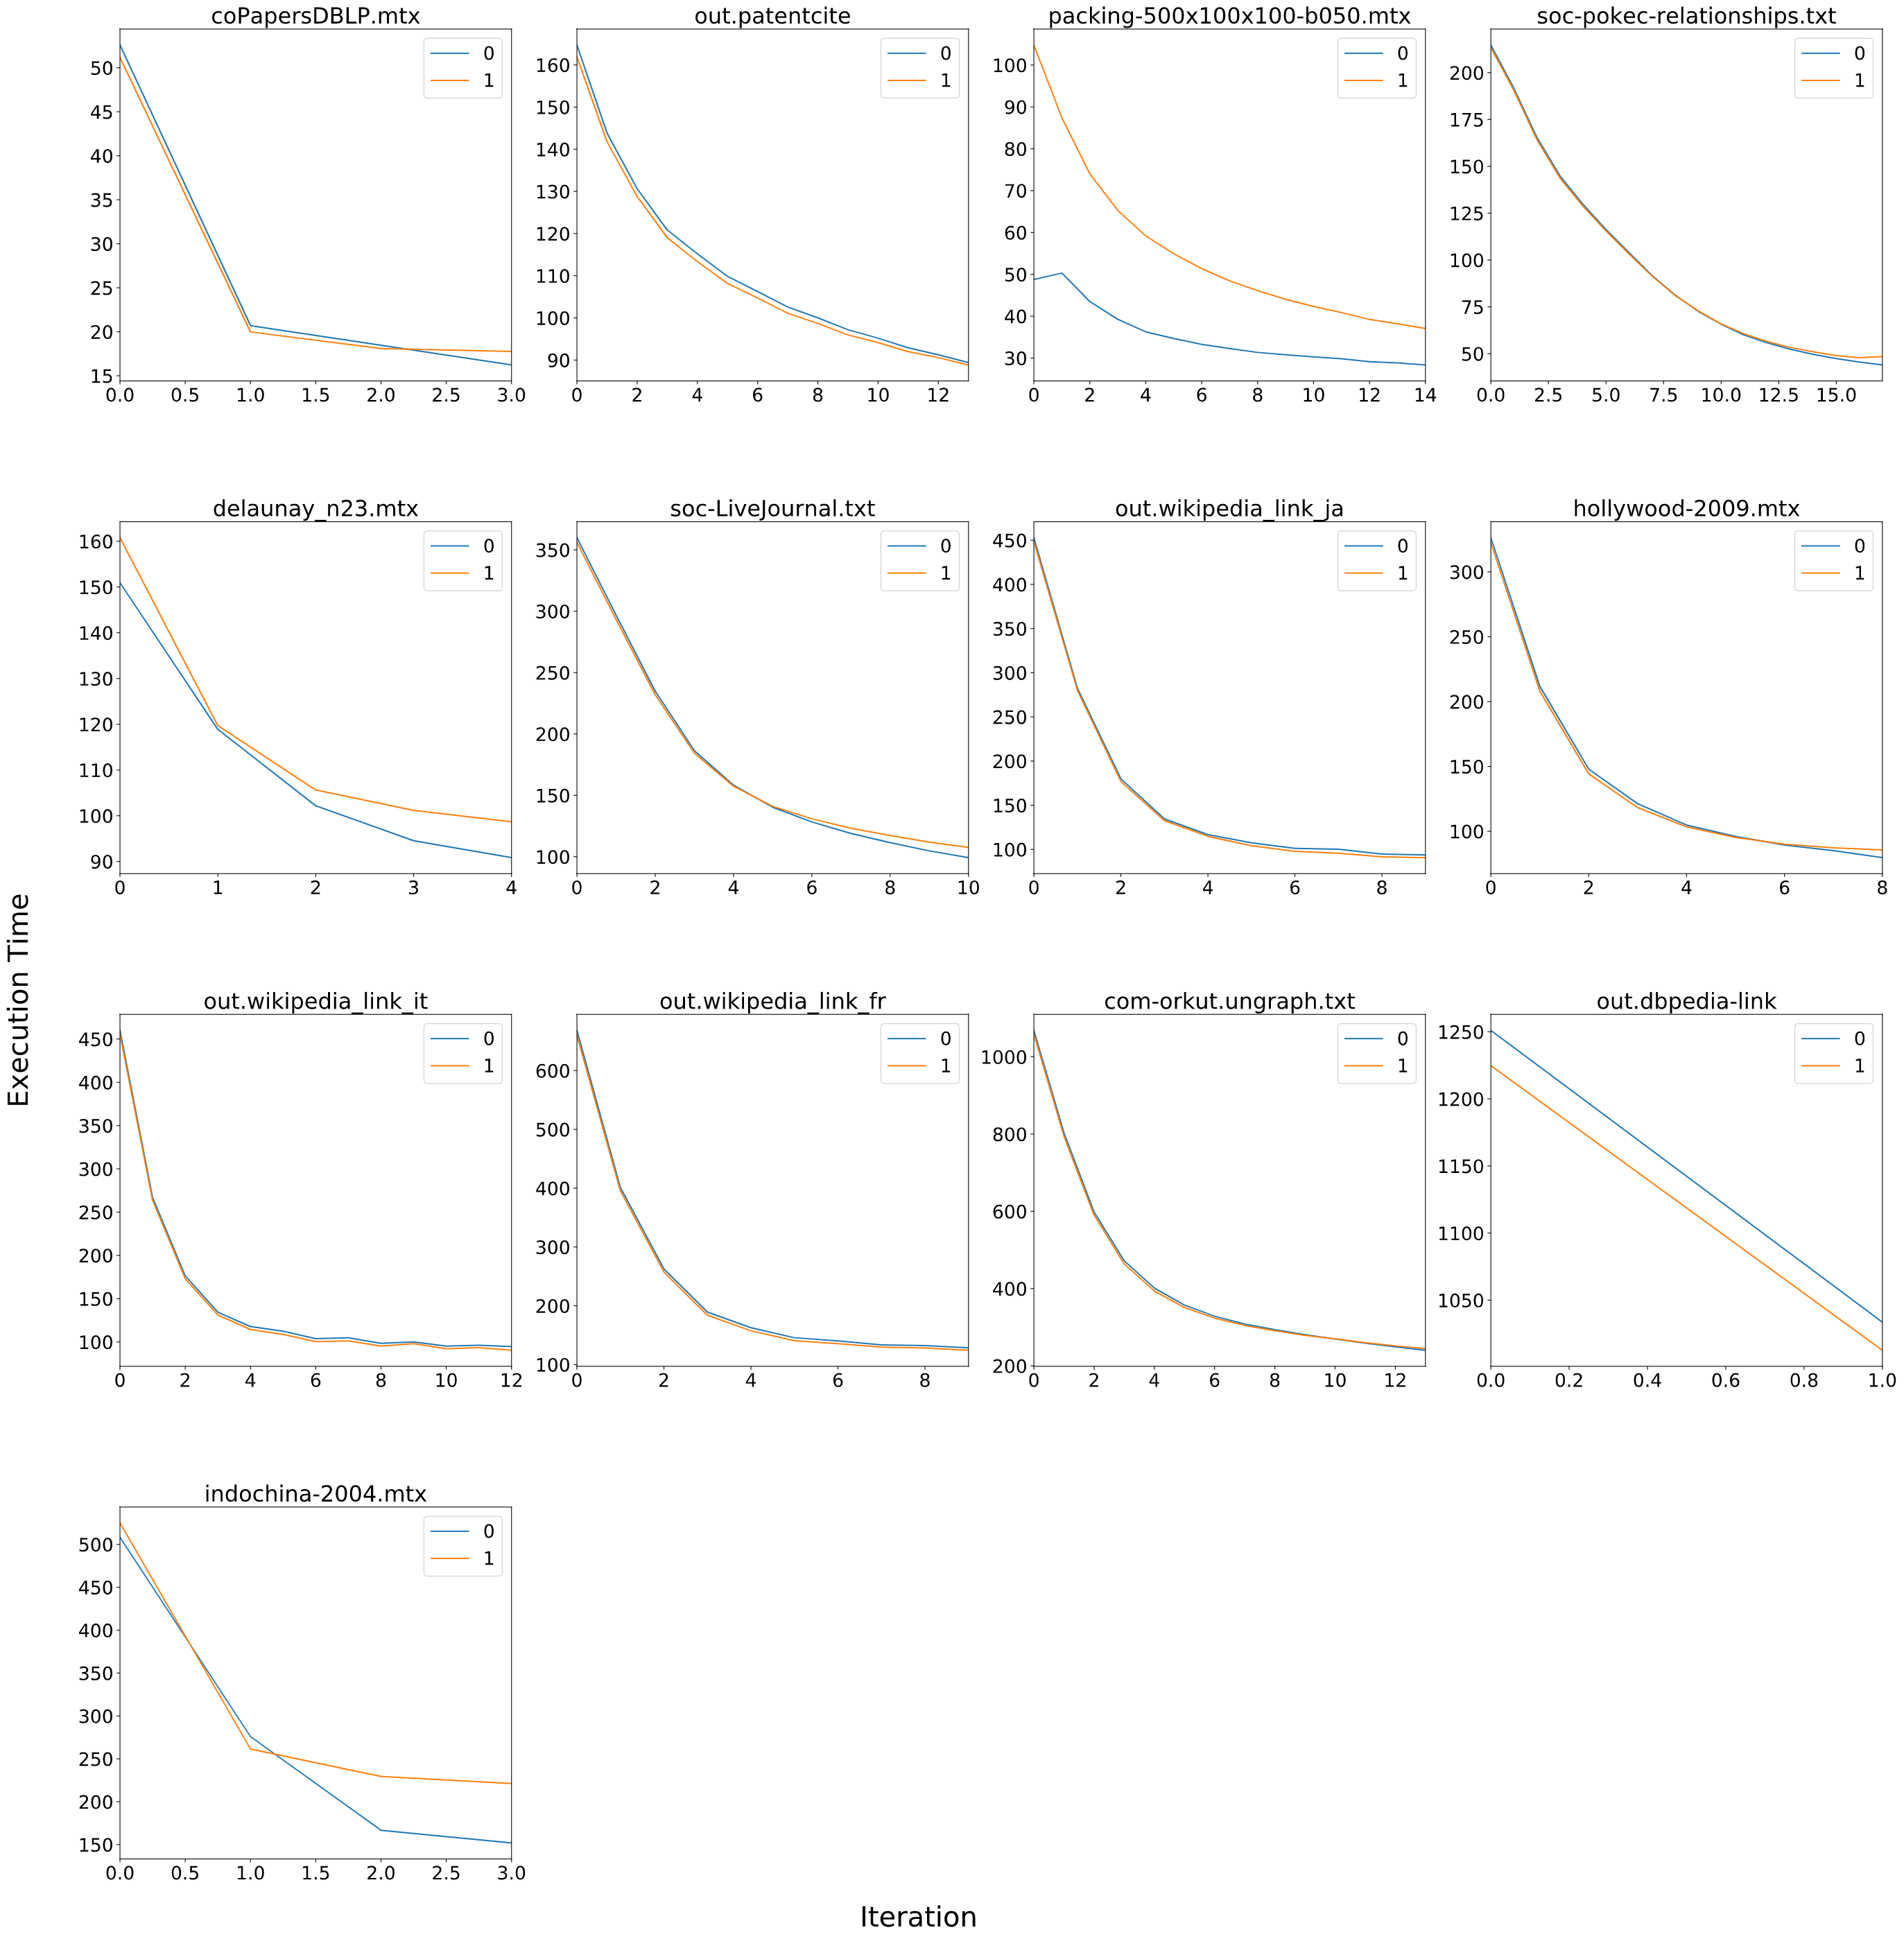
\includegraphics[width=1\linewidth]{0-resources/hash-prune-vs-no-prune}
	\caption{Comparison of the execution time between the Hashmap (in blue) and a version of comparison without the pruning approach (in orange) for each execution of the first optimization phase, excluding the first one. }
	\label{fig:hash-prune-vs-no-prune}
\end{figure}
\noindent We evaluate the impact in terms of time of the pruning approach in the PH-Louvain algorithm as before: we compare the algorithm with another test version in which we remove the pruning. In the Figure \ref{fig:hash-prune-vs-no-prune} there are the execution times of the first optimization phase for each iteration of both two versions. As previous, we exclude from this graphic the first iteration. \\
We notice that the two algorithms perform generally in a similar way, with a significant difference only when the pruning reduce considerably the number of edge: the pruning algorithm is slower up to $\sim25$ ms at iteration (in the graph dbpedia-link), caused by the extra time to compute the pruning information. Even if reducing the number of edges analyzed reduce the execution time, the gap between the two version is not directly proportional with respect to the number of edges pruned like in the previous version: this is due to the the branching problem for thread in the same warp. \\
During the Fill Map sub-phase, we insert in the map each pair node-community such that the nodes has almost one neighbour that change community in the previous iteration.
To perform this operation, an edge $(source, destination)$ is assigned to each thread: than it check if the source node match the pruning requirement, it change the destination node with the destination communities and insert the value in the map. If an edge has a source node that doesn't match the criteria, its thread will return without doing nothing else. The problem is that the nodes are organized in warp of 32 threads assigned to a core of the Streaming Multiprocessor: the GPU execute a new warp on the same core only when all thread of the old warp finish the execution. If in a warp there is even just one thread that have to insert the pair in the map, all the other thread have to wait it. This reduce the gain in terms of times in the Fill-Map sub-phase.
\begin{figure}[t!]
	\centering
	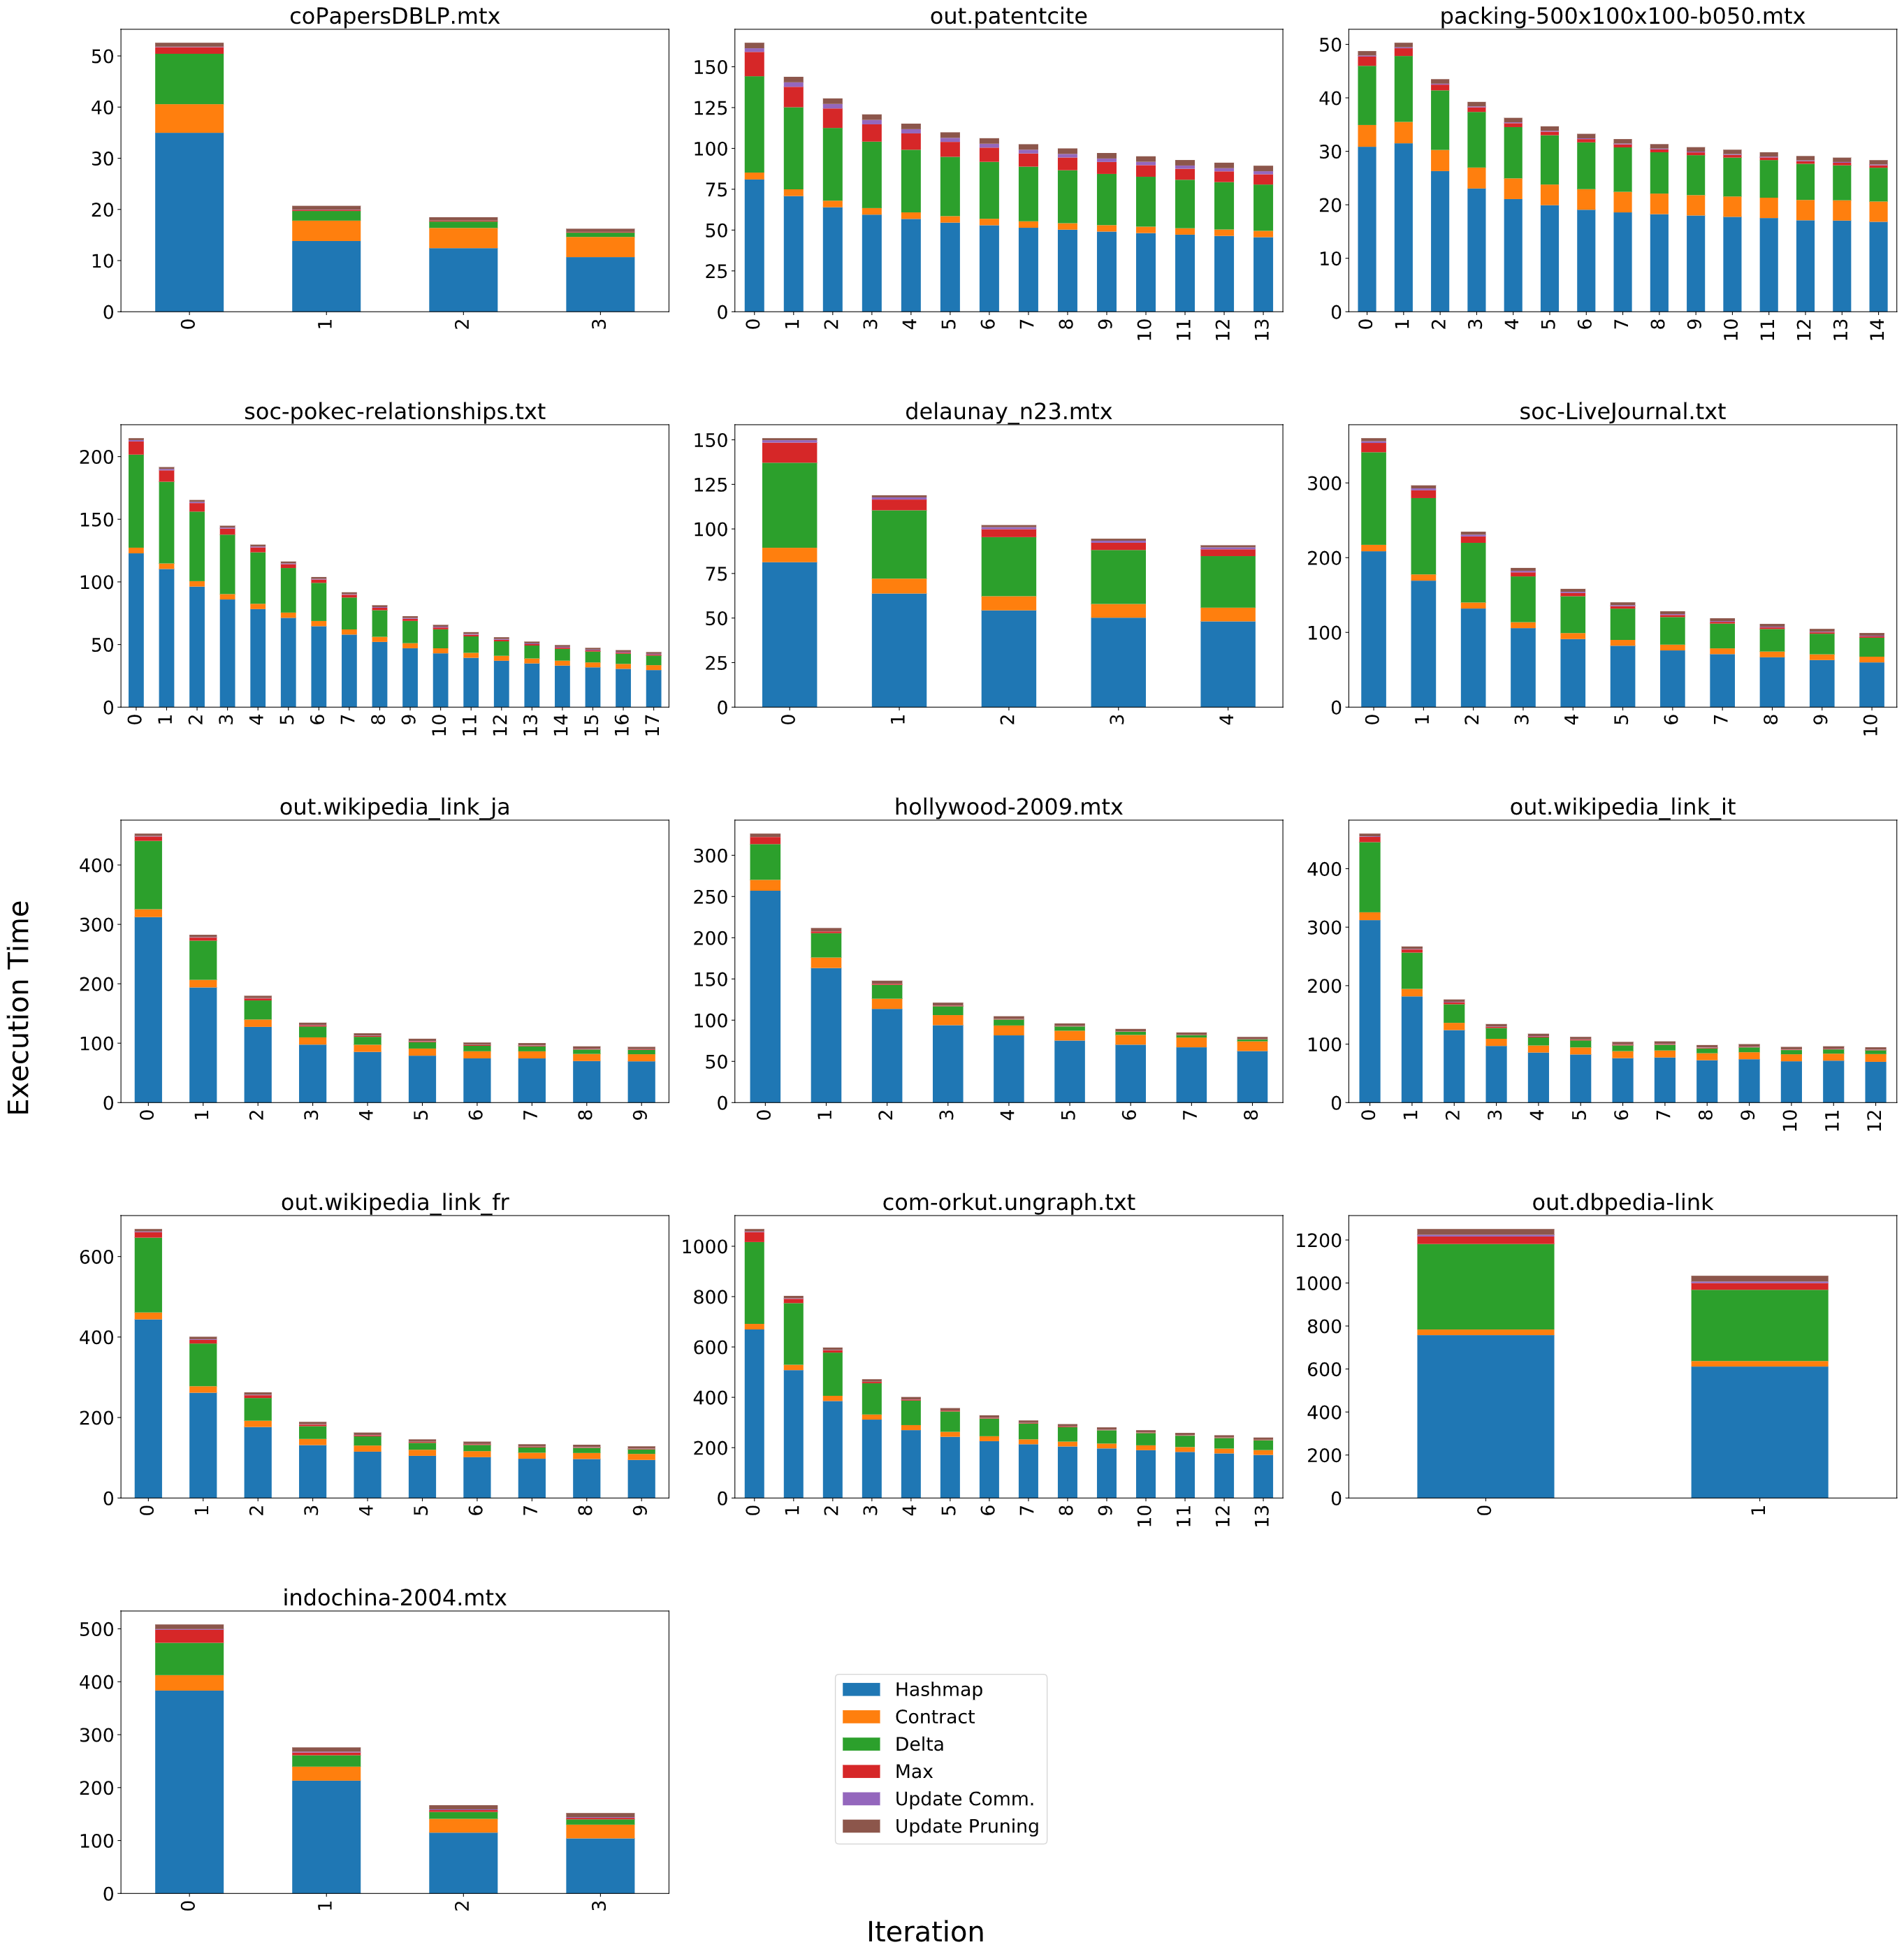
\includegraphics[width=1\linewidth]{0-resources/suphases-hash}
	\caption{}
	\label{fig:suphases-hash}
\end{figure}

We notice that in the no-pruning version the execution time tend to decrease even in the case in which the pruning doesn't remove a considerable part of the edges (like the wikipedia\_link\_jp dataset), so we analyze the sub-phases in order to see what change between each iteration: in the Figure \ref{fig:suphases-hash} is illustrated the consuming time of each sub-phase with respect to the total time of each iteration.
The most consuming sub-phase is the fill map:  this sub-phase at least 50\% of the time, reaching peek of even more than 75\%. We notice that at each iteration, the times required decrease: therefore we focus our analysis on this behaviour of the map. We analyze the number of conflict that we have when we try to insert a new key in the map. 
We notice that, iteration by iteration, the number of conflicts in the map decrease: the reason is that, at each iteration, the number of different key inserted decrease. Indeed, at every iteration the number of communities decrease because similar nodes tends to converge to one community for groups: this reduce the number of possible different keys node-community that we have. 
Then, we analyze the number different keys inserted in the map at each iteration.\\
\begin{figure}[t!]
	\centering
	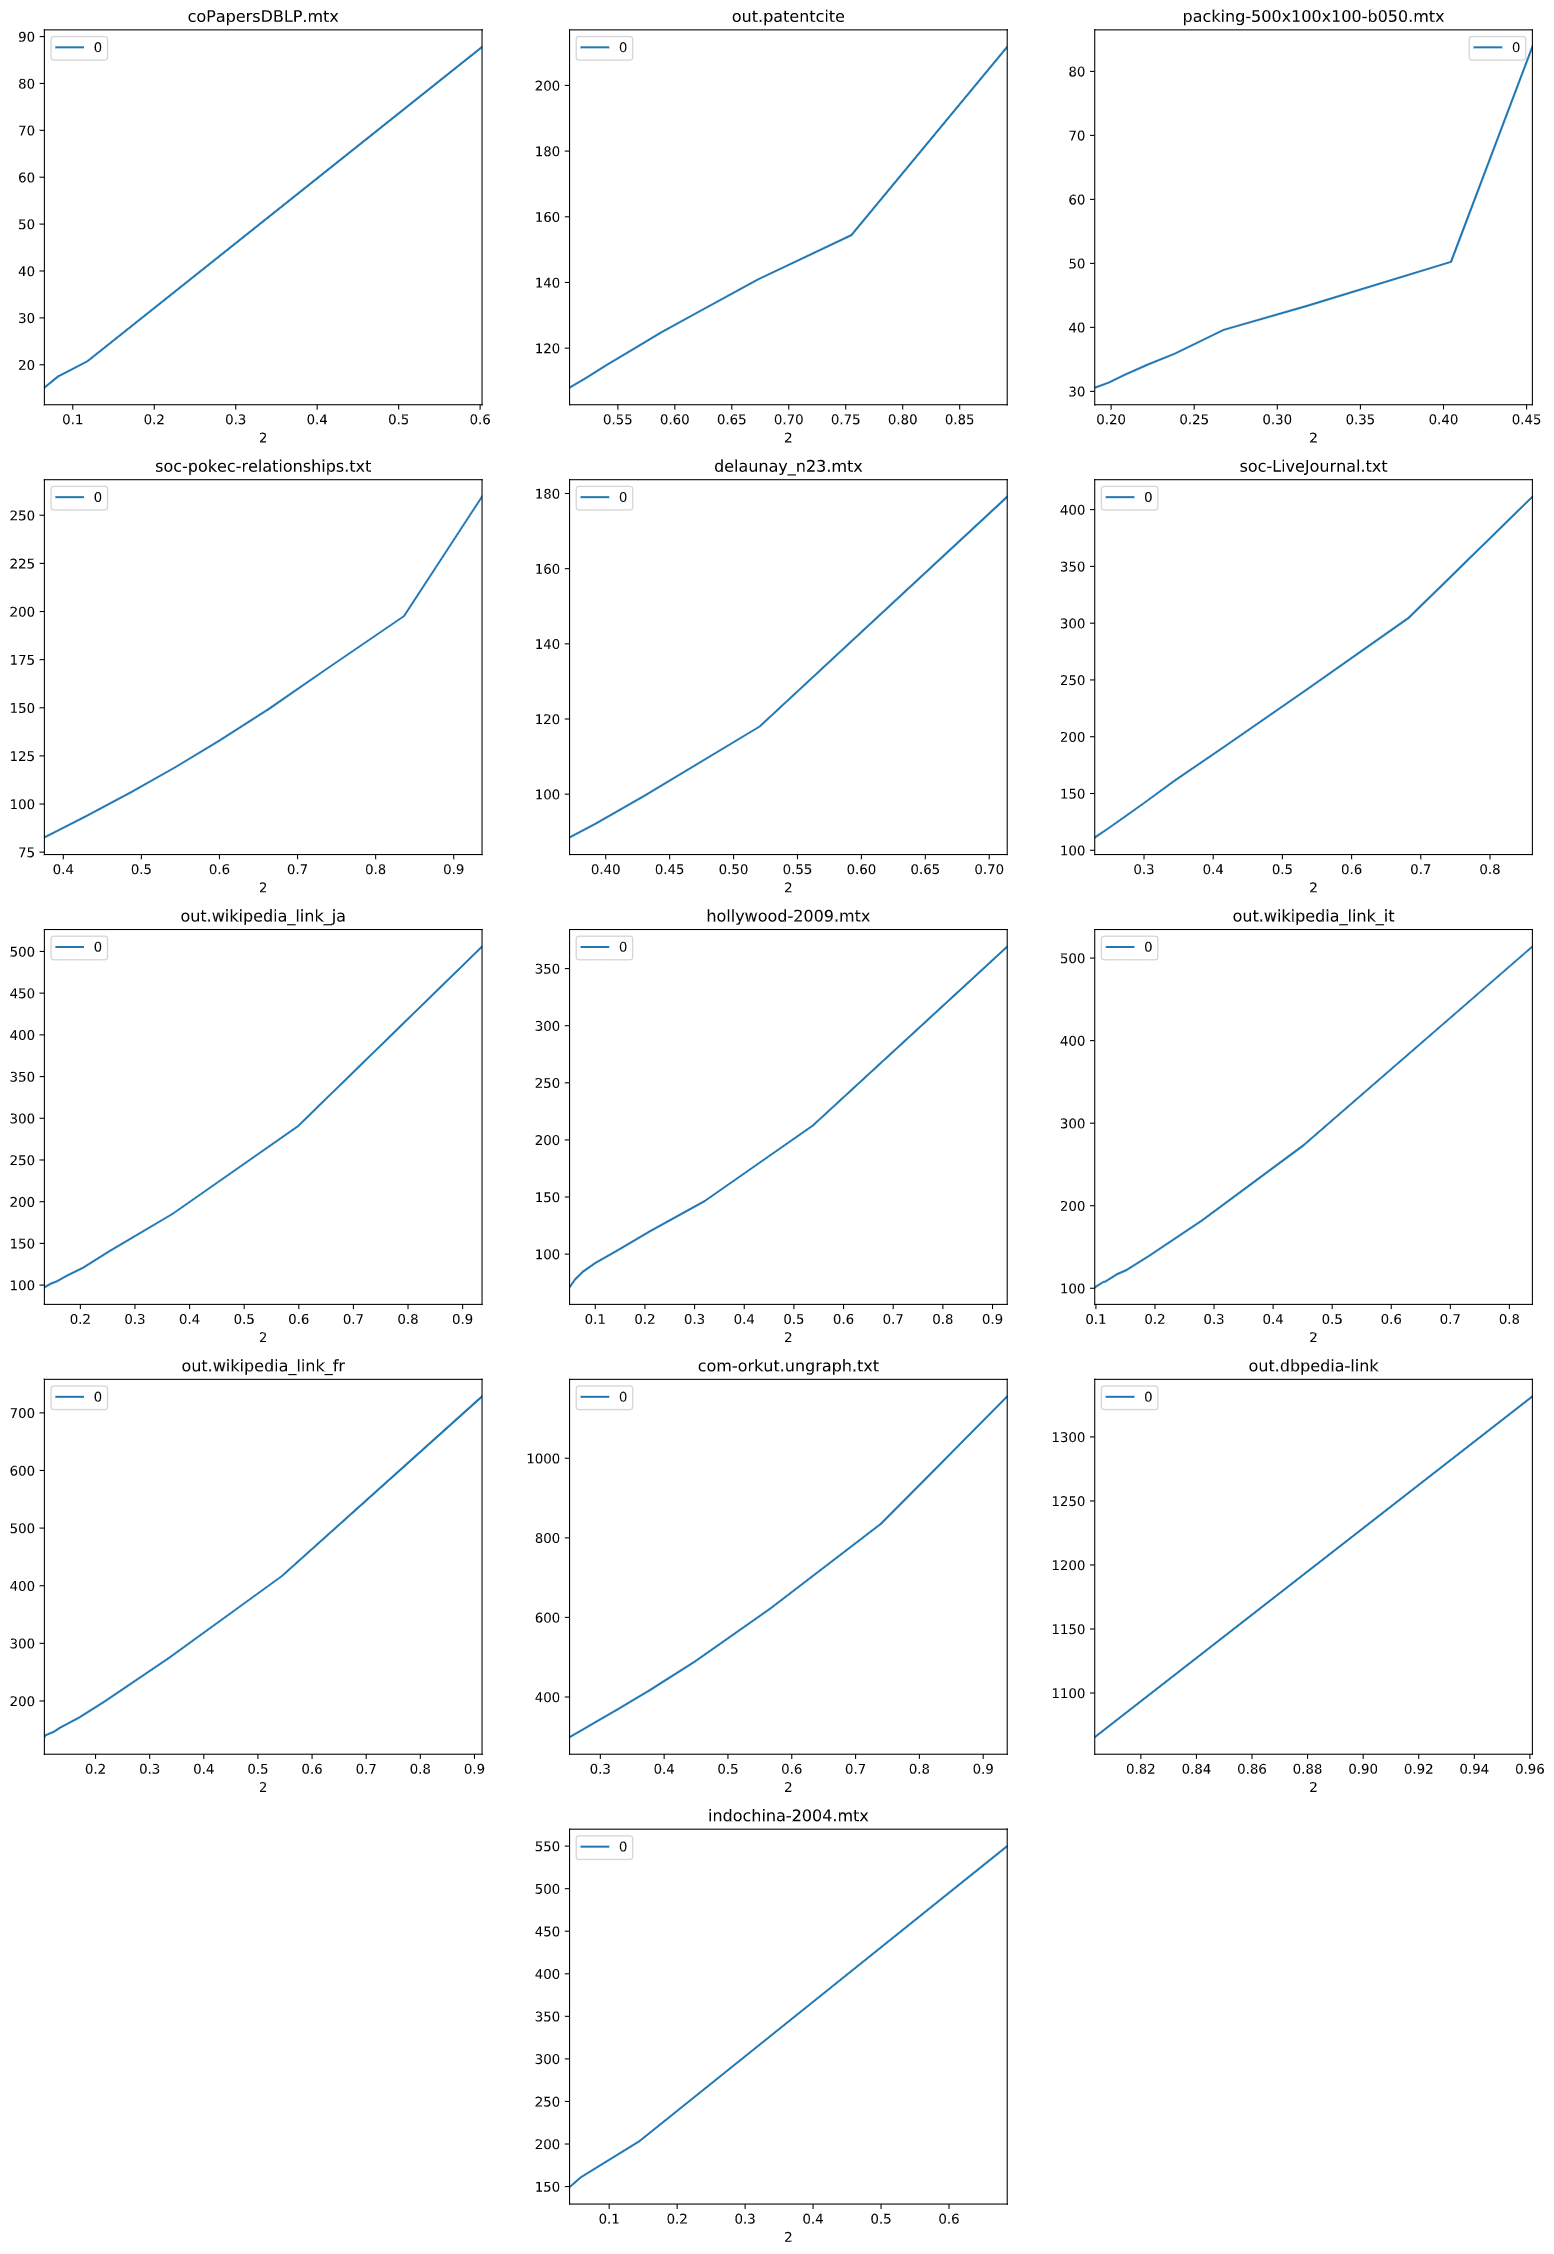
\includegraphics[width=0.7\linewidth]{0-resources/time-vs-possible-keys}
	\caption{Execution time of the Hashmap version in relation to the number of different pair (node, community) inserted (expressed with respect to the maximum number of keys).}
	\label{fig:time-vs-possible-keys}
\end{figure}
\noindent In the Figure \ref{fig:time-vs-possible-keys}, we have on the x-axis the number of different keys at that iteration with respect to the maximum possible number of keys (i.e. the number of edges, because we have the maximum when each node is in its self-community); on the y-axes we have the execution times. We notice that there is a direct correlation between this data and this two values, and this explains why the PH-Louvain algorithm performs better in the last iterations with respect to the first ones. 
\newpage
\subsection{Algorithms comparison}\label{alg-comp}
\begin{figure}[h]
	\centering
	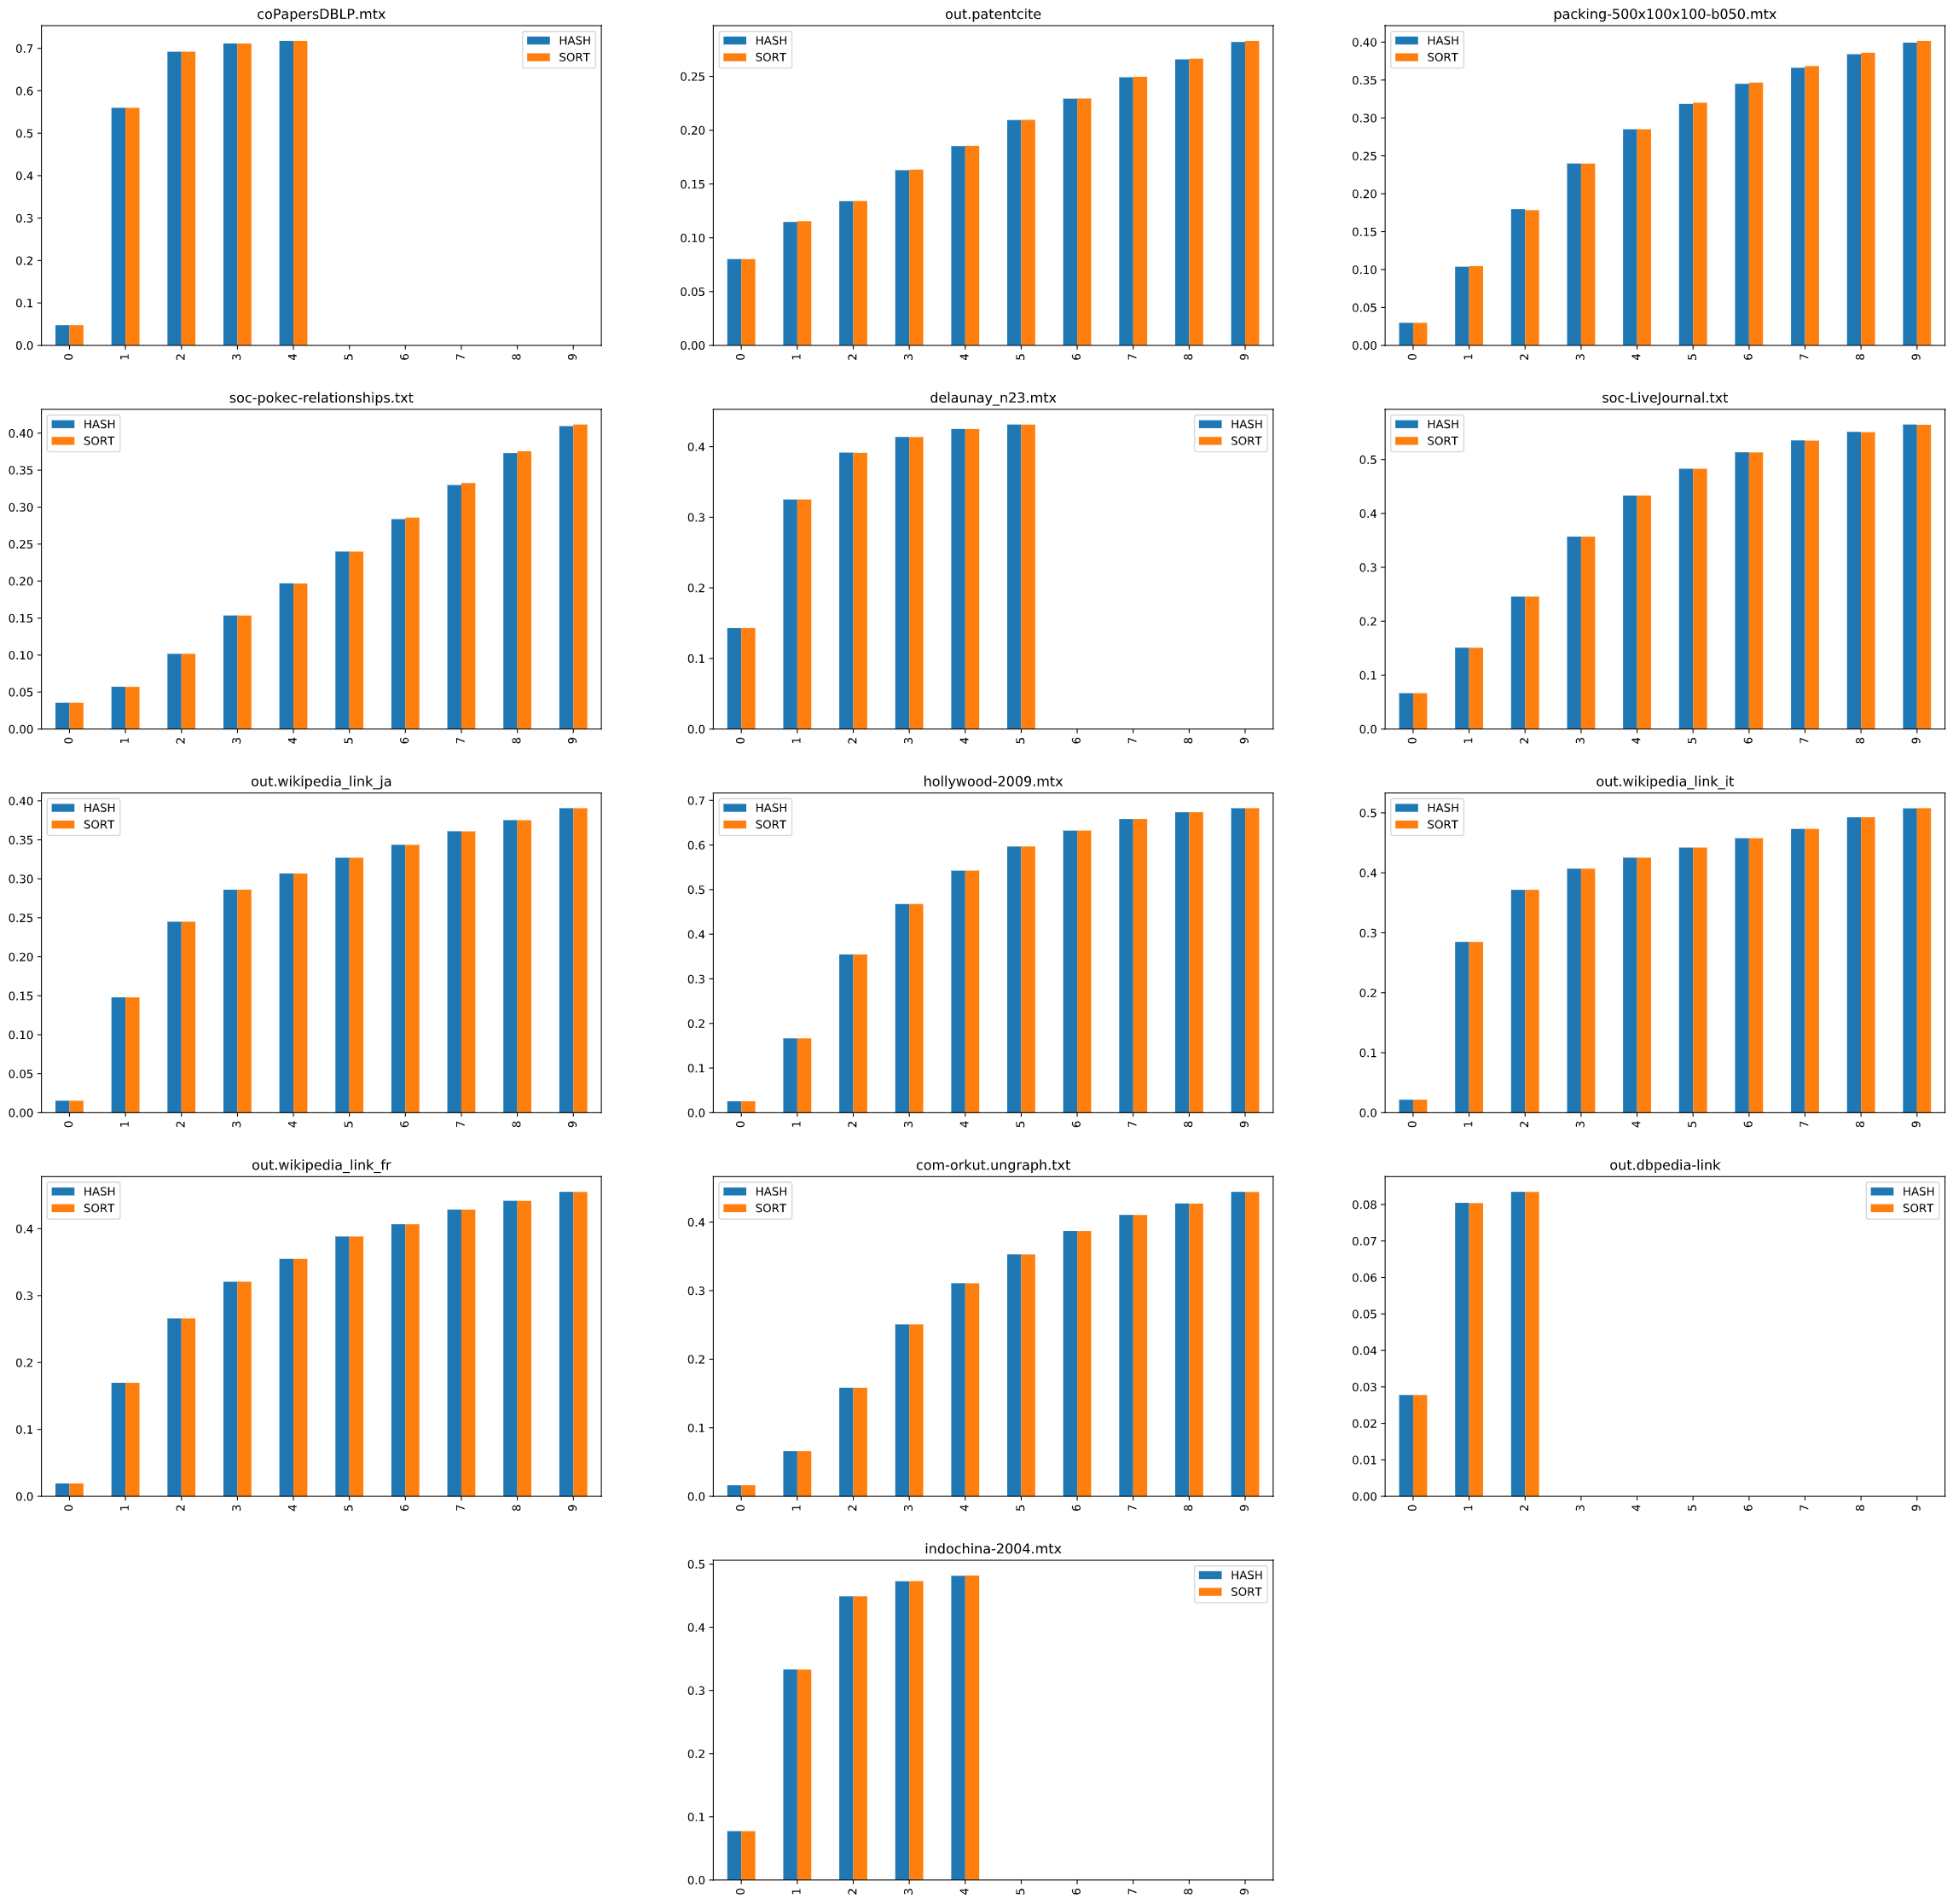
\includegraphics[width=1\linewidth]{0-resources/modularity-progression}
	\caption{Modularity Progression in the first ten iteration of the optimization phase.}
	\label{fig:modularity-progression}
\end{figure} 
\noindent In this section, we focus our analysis on the comparison between the two algorithm in order to find advantages and disadvantages of each method. 
First of all, we notice from the Table \ref{tab:mod} that the two algorithm obtain a very similar score of modularity. In the Figure \ref{fig:modularity-progression}, we expose the progression of the modularity $Q$ in the first operation. As we can see, the modularity in the two algorithms grows in almost identical way: this is due to the minimum labelling heuristic (Chapter \ref{parallel-imp}) that force the algorithms to converge to a similar result. \\
\begin{figure}[t!]
	\centering
	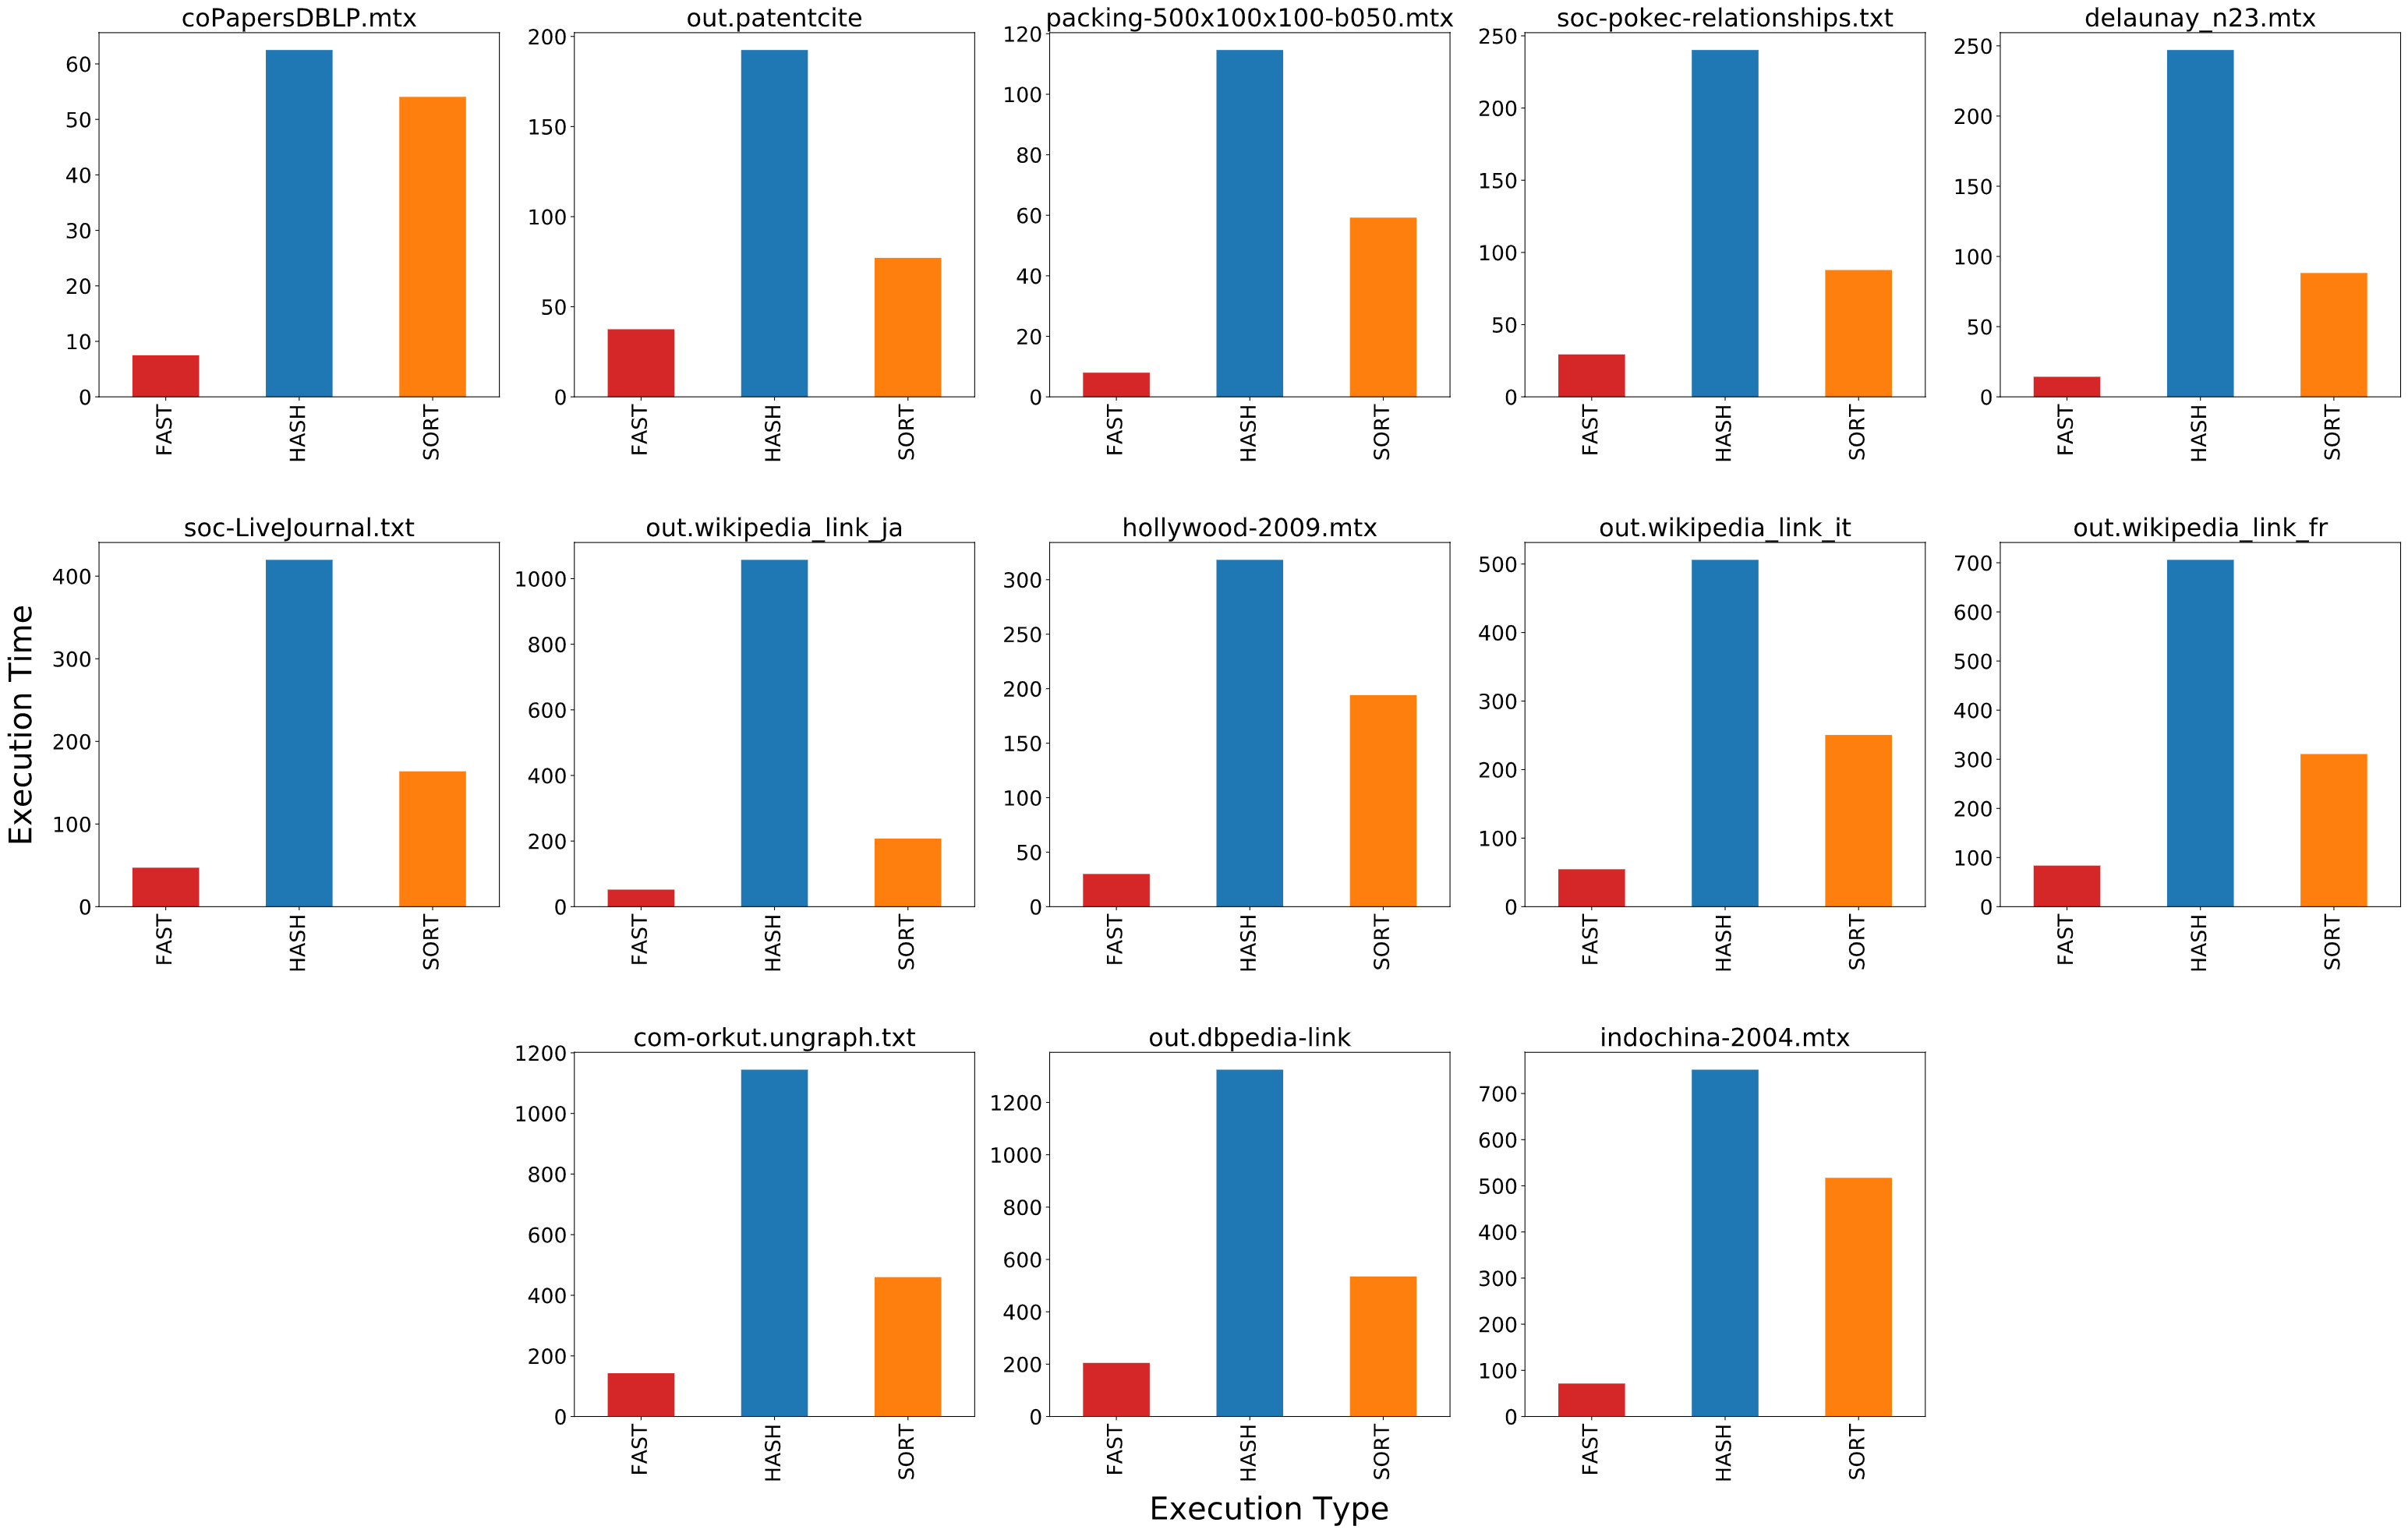
\includegraphics[width=1\linewidth]{0-resources/first-hash-sort}
	\caption{Comparison of the execution time of the first iteration of the first optimization phase between the two presented versions unoptimized of the algorithm and the optimized version.}
	\label{fig:first-hash-sort}
\end{figure}
To analyze the differences in terms of performance, we start analyzing the impact of the optimization of the first iteration of the optimization phase for both the algorithms. We are expecting an huge reduction in terms of times, considering that we remove the most consuming time phase from the Prune-Sort-Reduce routine, i.e. the sorting phase. As shown in the Figure \ref{fig:first-hash-sort}, we obtain the expected results: we obtain a reduction in range between $\sim 51\%$ and $\sim 86\%$ respect to the PSR-Louvain and a reduction in range between $\sim 84\%$ and $\sim 95\%$ respect to the PH-Louvain. From the data we also see that in the second algorithm, this optimization introduce a little delay in the next iteration respect to the first one: this is caused by the deallocation of the support variable used in the fast approach (that are the same used in the PSR-Louvain) and the allocation of the hashmap and other support variables. But, this overhead is much smaller than the gain obtained by the optimization, therefore we consider it a valid technique to improve the performance.\\
From the Figure \ref{fig:first-hash-sort}, we also note that the PH-Louvain is always slower with respect to the PSR-Louvain, and for this reason this technique has a greater impact on it. Considering this particular feature, we choose to go further in our analysis: we compare the iterations of the first optimization phase in terms of times of the two version of the algorithms, excluding the first iteration.
\begin{figure}[t!]
	\centering
	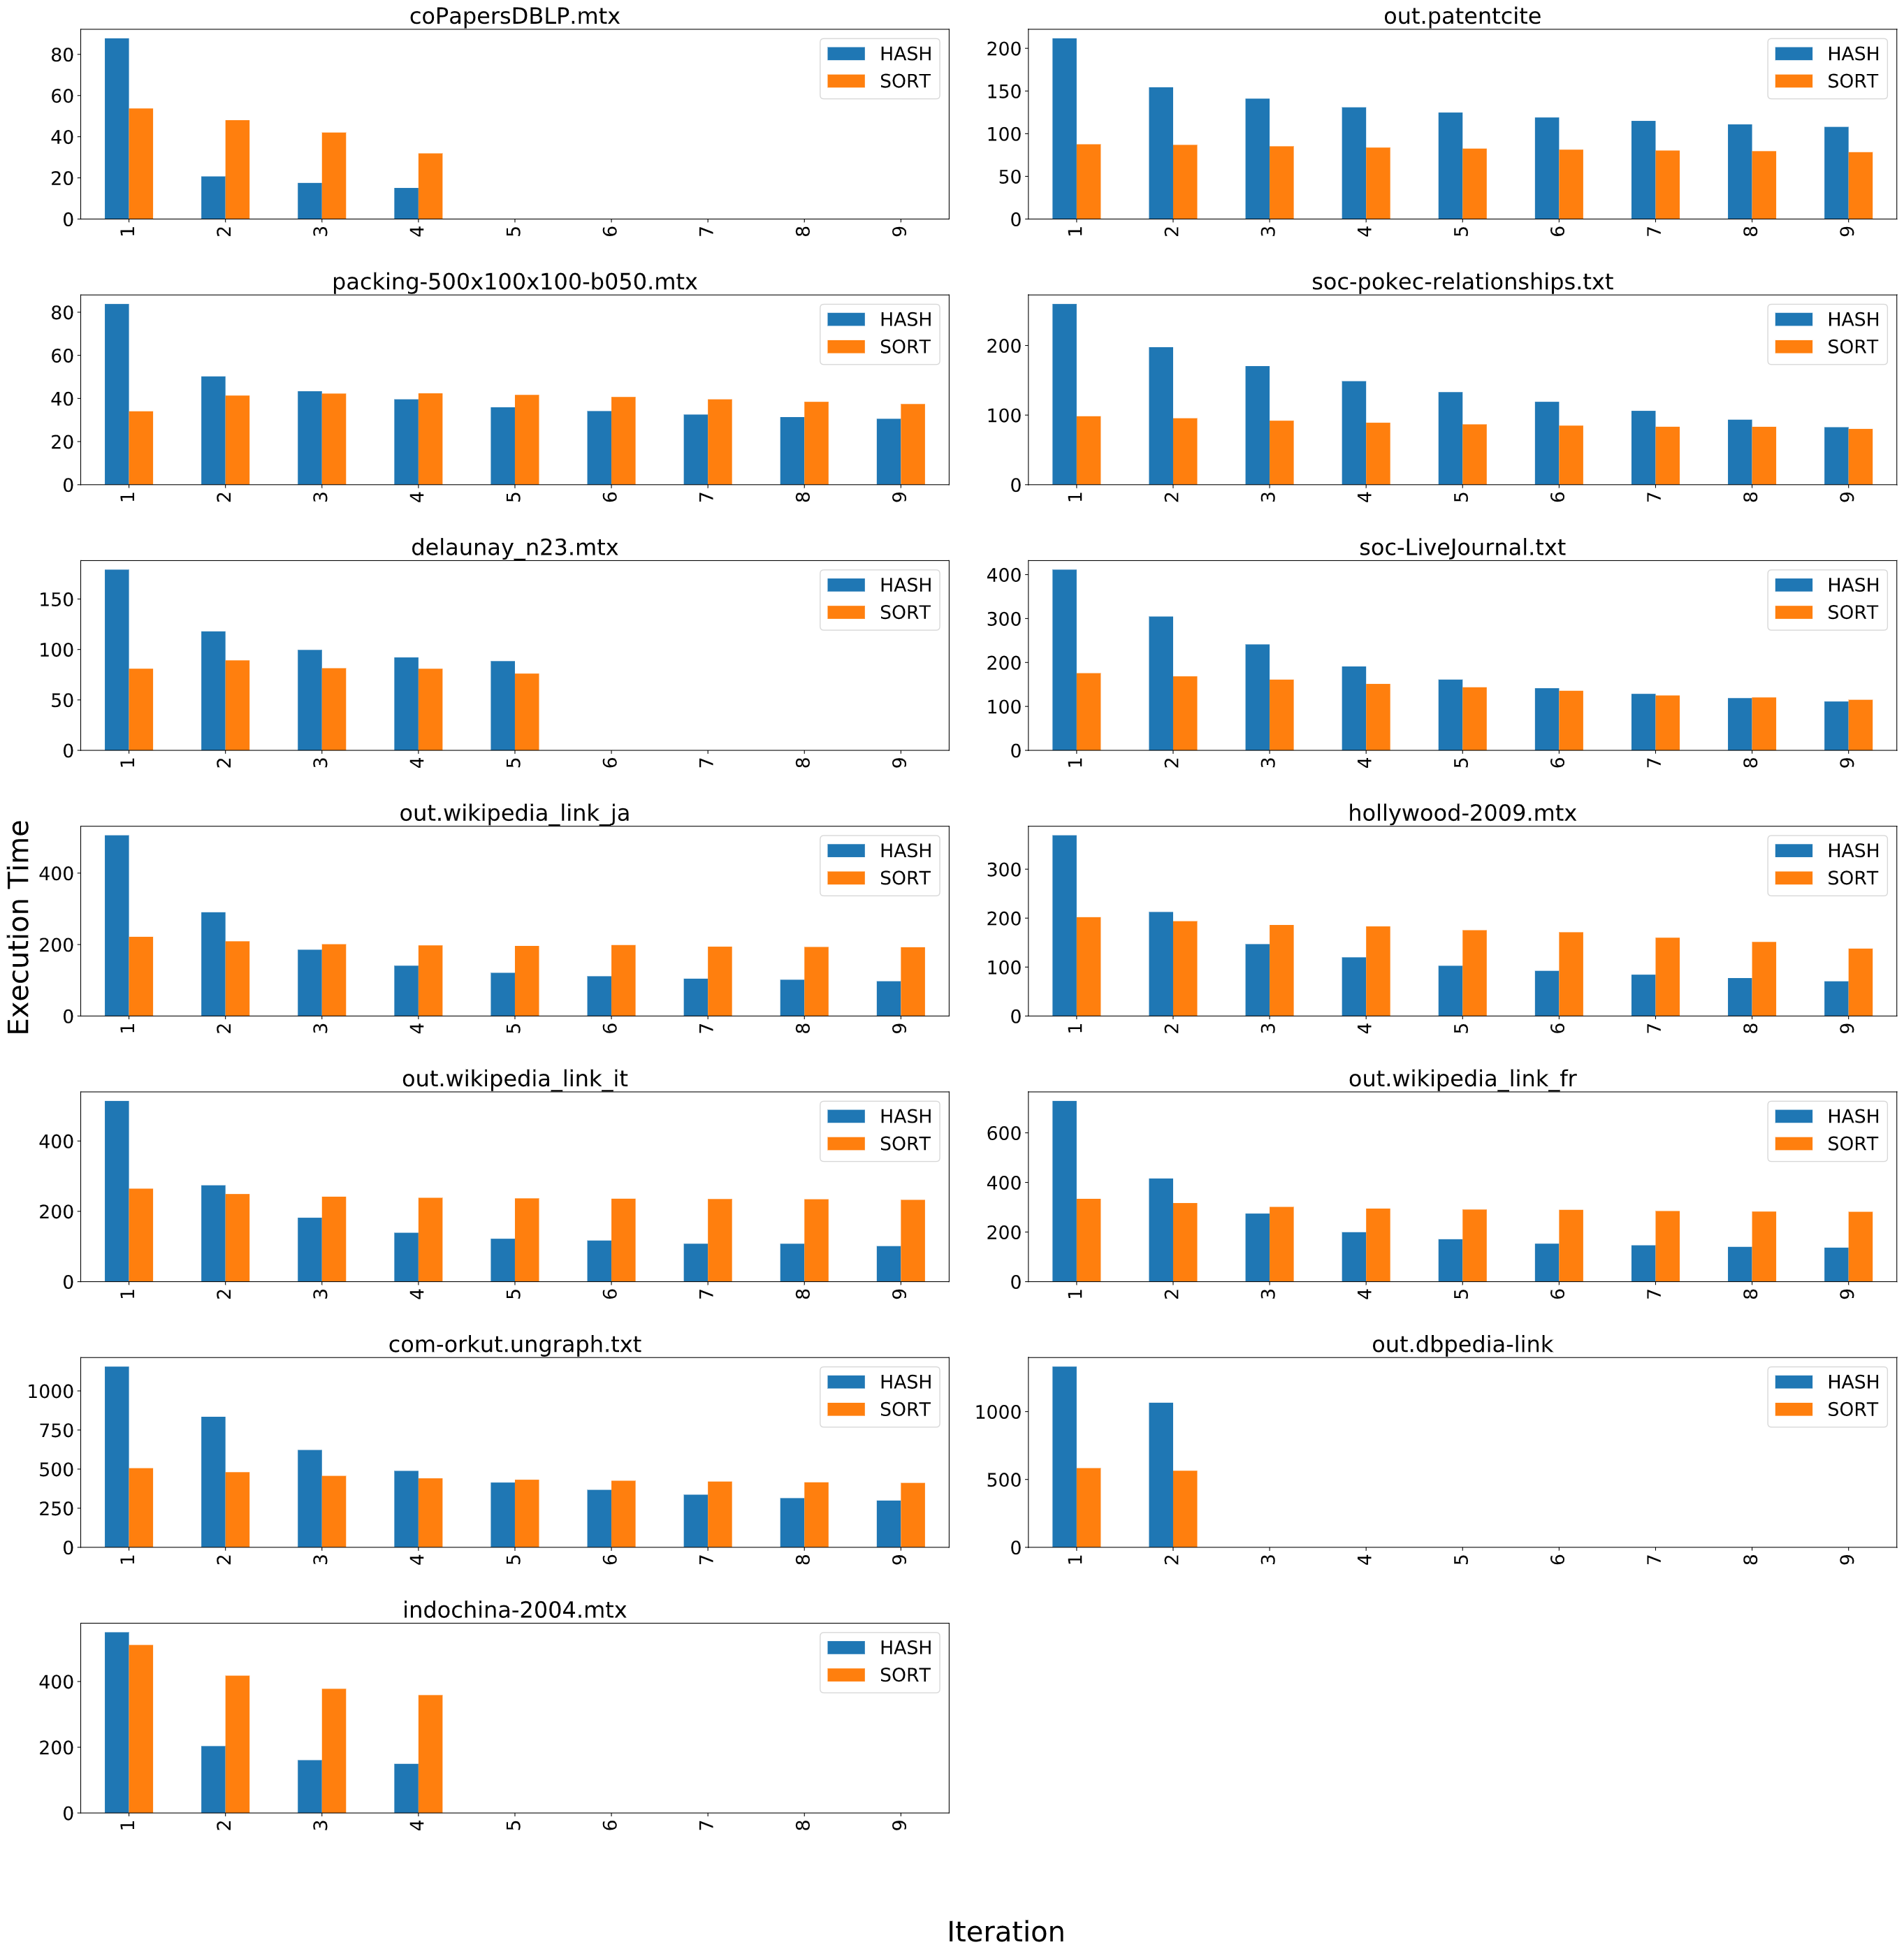
\includegraphics[width=1\linewidth]{0-resources/hash-vs-sort}
	\caption{Execution time in the first ten iteration of the first optimization phase, excluding the first optimized iteration.}
	\label{fig:hash-vs-sort}
\end{figure}
In the Figure \ref{fig:hash-vs-sort} are exposed the results. We notice that the second iteration of the PH-Louvain is always slower respect to the PSR-Louvain.
Considering the observation presented in the previous chapter, we conclude in the first iterations the PH-Louvain algorithm suffer respect to the other due to the high number of different pair key-community that we insert in the map. 
On the other hand, if the number of different pair drops below a given values, the hashmap performs better.
Instead, the PSR-Louvain does not benefit from a similar behaviour and its performances are generally more stable (they are improved consistently only by the pruning). 
We analyze in a similar way also the other optimization phases (Figure \ref{fig:multi-phase:optimization}). 
We notice that, from the second optimization phase, generally the PSR-Louvain performs better in terms of total time (i.e. sum of the time of each iteration) than the PH-Louvain: this because the number of iteration generally decrease phase by phase and the first approach generally performs better than the second one in the first iterations of the phase. Even if the number of conflicts decrease (due to the fact that we allocate in a map with the same order of magnitude of the first phase in the following phases), also the time of the sorting sub-phase of the other algorithm decrease: to really see an improvement of the hashmap respect to the other approach we a similar convergence see in the first optimization phase.
For these reasons the sorting version of the algorithm tend to perform better than the hashmap one from the second optimization phase. \\
We study also the difference between the algorithms in terms of aggregation phases: the results of our study are presented in Figure \ref{fig:multi-phase:aggregation}.
We notice that the execution times of the PH-Louvain tend to perform better with respect to the PSR-Louvain. Considering the observation about the performance of the hashmap that we make previously, its easy to motivate this performance results: the hashmap perform better respect to the sorting approach when the number of keys decrease consistently. In the aggregation phase, the number of the active communities is decreased compared to the starting situation. Besides, in this phase we insert in the map a key composed by the two communities id: this involves a further reduction of the number of keys inserted, because we tend to insert more often the same key in the map. Therefore the performance are related to the number of different active communities find at the end of the optimization phase: indeed the only two case in which the sort-reduce version perform better with respect to the hashmap version are those in which the number of communities is decreased slightly with respect to the number of edges (i.e. the maximum possible number of communities).
All of these consideration are at the base of the design of an adaptive approach that we present in the next section: indeed, we can estimate if the PH-Louvain performs better then the other algorithm by the comparing of the number of different keys with respect to the number of the possible one, and select the right algorithm to use.	
\begin{figure}[t!]
	\hspace*{-4em}
	\subcaptionbox{\label{fig:multi-phase:optimization}}{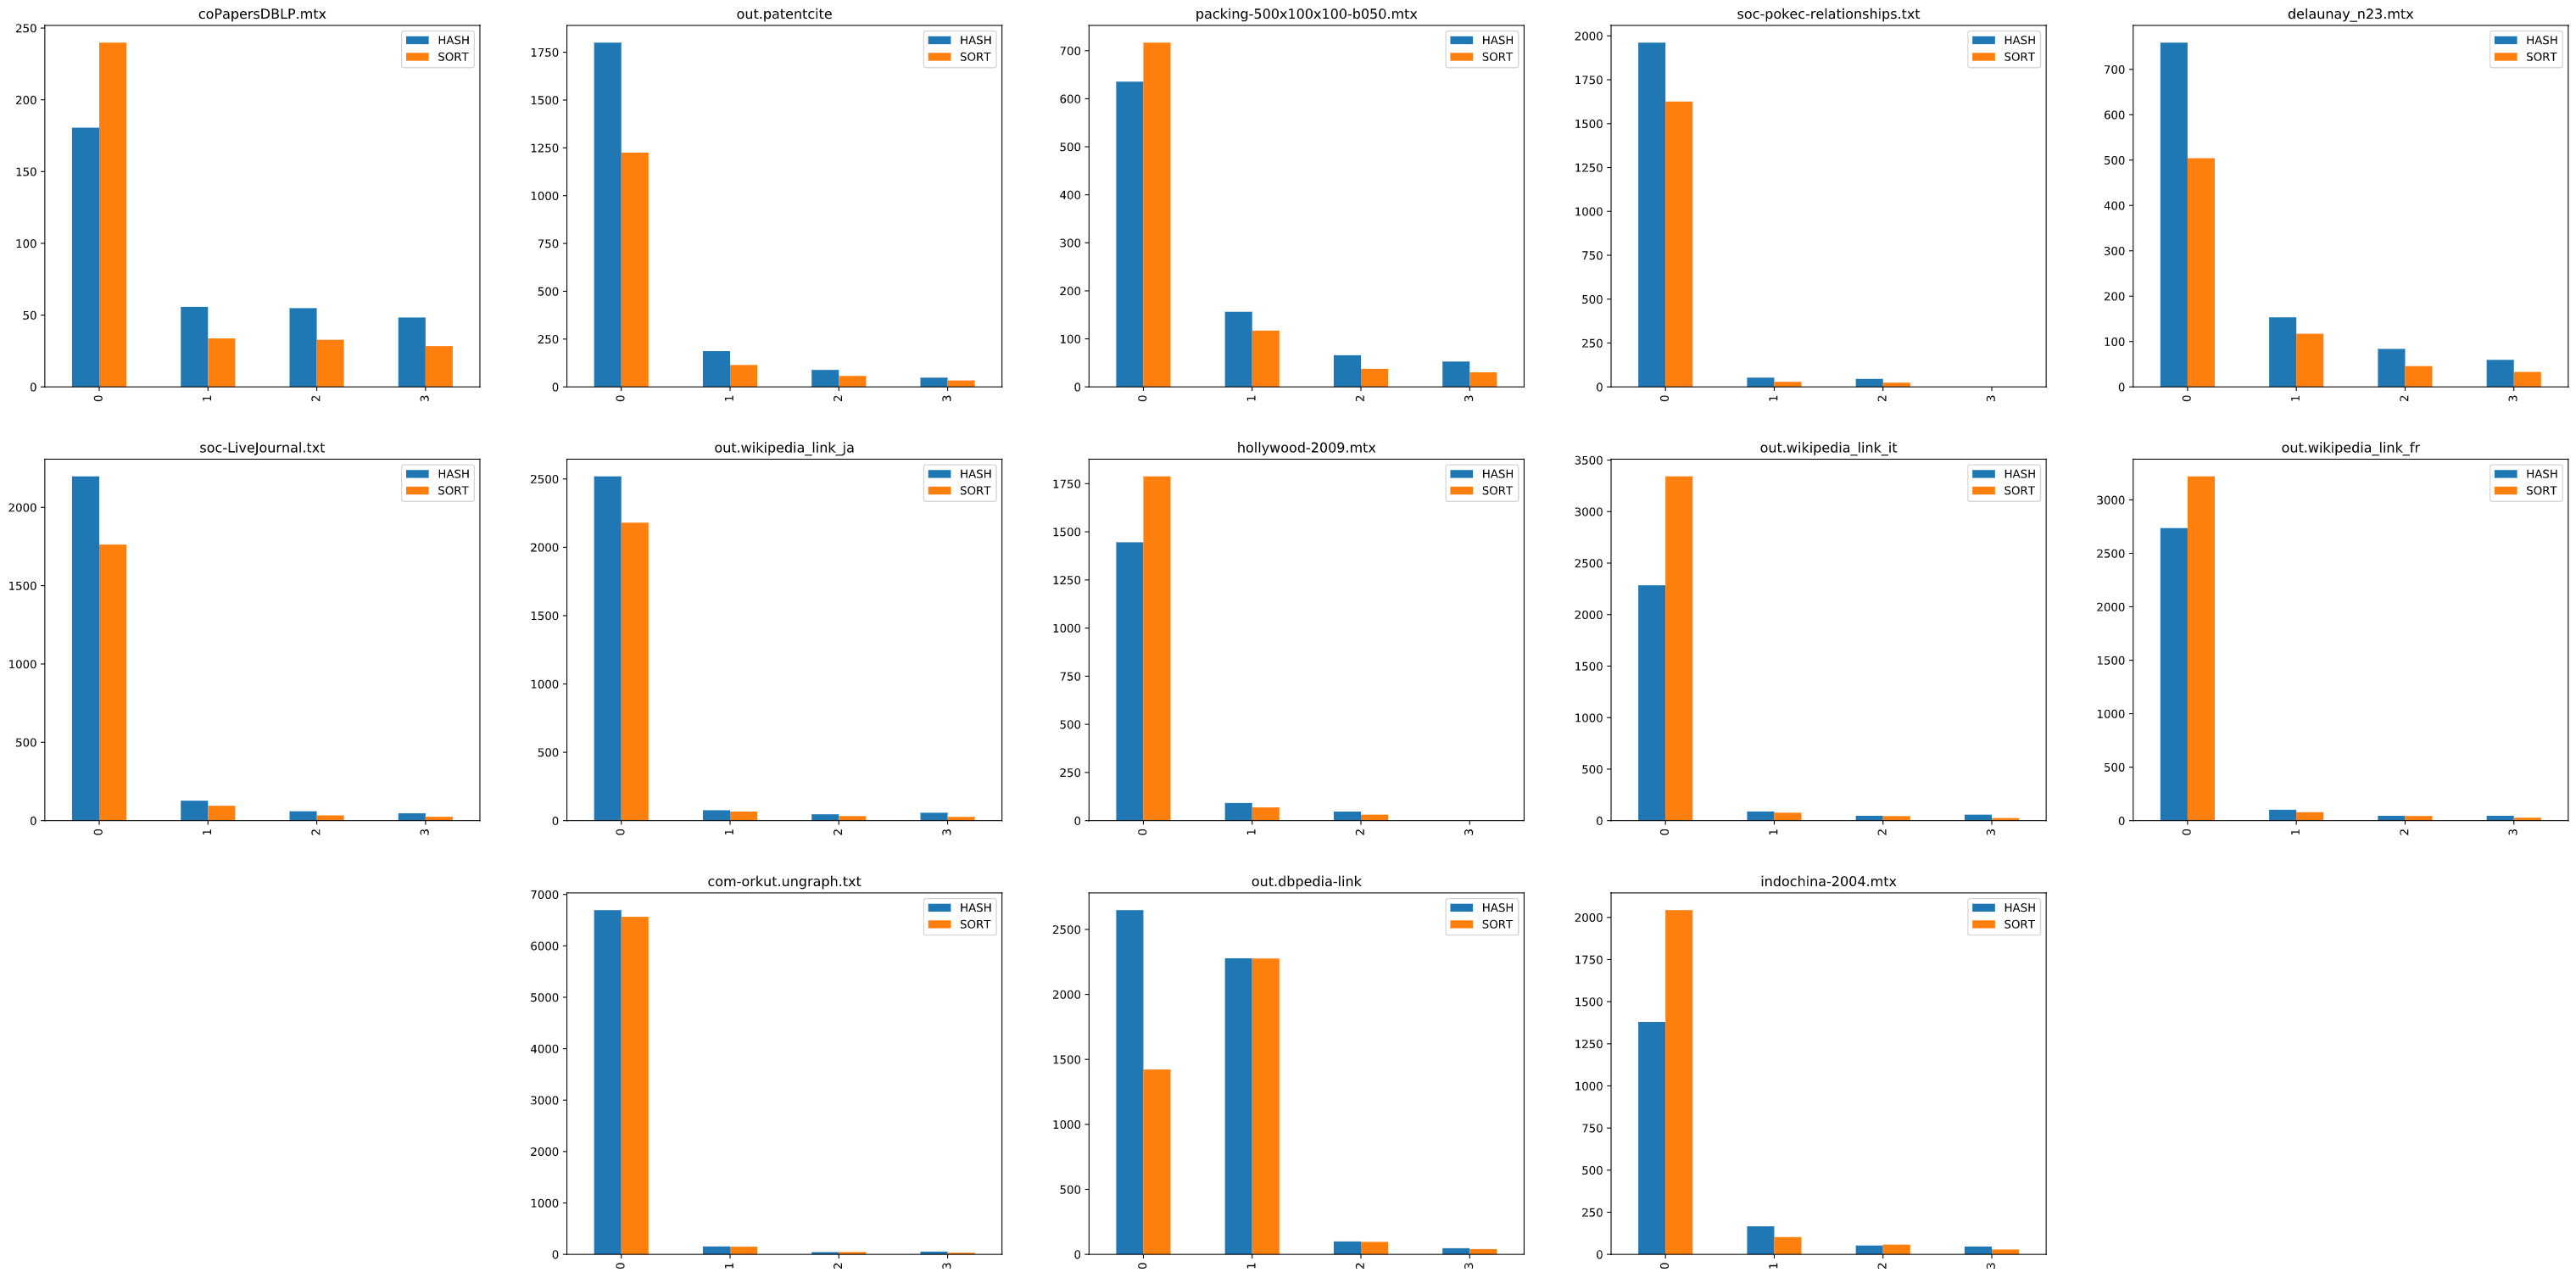
\includegraphics[width=0.6\linewidth]{0-resources/optimization-phases.png}}
	\hspace{2em}%
	\subcaptionbox{\label{fig:multi-phase:aggregation}}{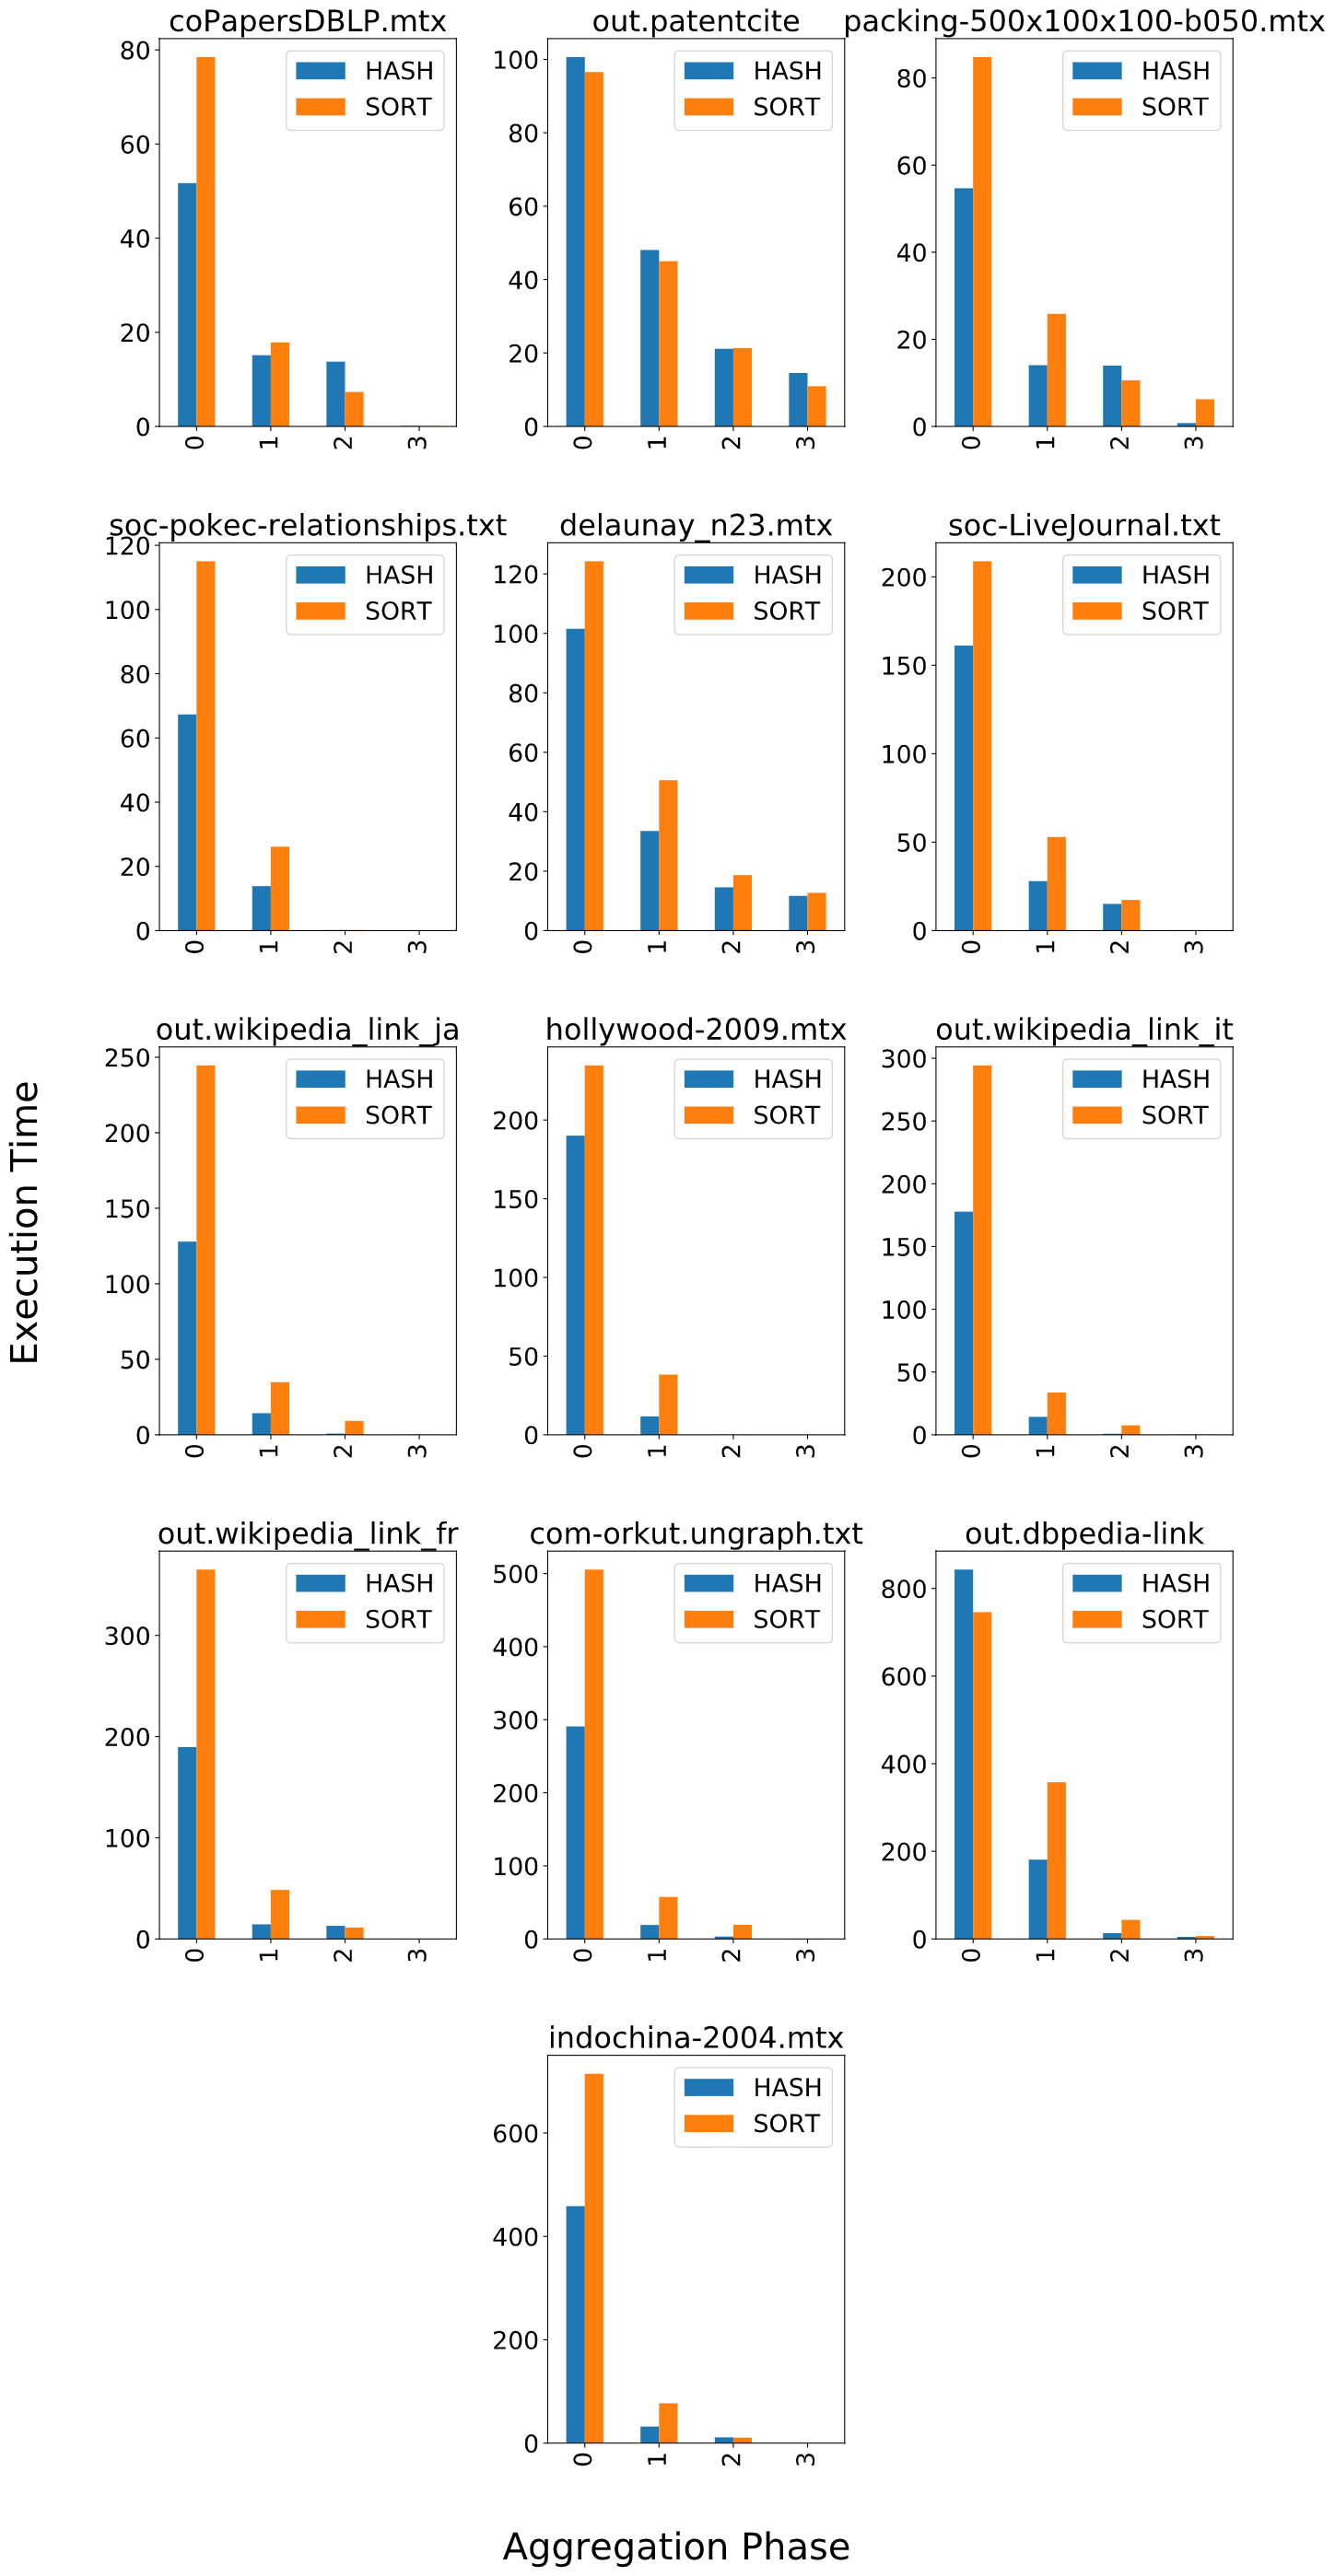
\includegraphics[width=0.6\linewidth]{0-resources/aggregation-phase.png}}
	\caption{(a): Execution times of the first four optimization phases;\\(b) Execution times of the first four aggregation phases.}
\end{figure}
\newpage
\section{Adaptive Louvain Algorithm}
In this chapter we finally present the adaptive algorithm: it uses an heuristic to switch from the sort-reduce version to the hashmap version when the number of different node-community keys falls below a certain threshold. This threshold is calculated in percentage with respect to the total number of possible keys, i.e. the number of edges.
Next, we make a comparison between our adaptive algorithm and other two Louvain algorithms for the GPU already available in two important libraries: the first one is included in the NVIDIA's cuGraph library; the second one in the Gunrock library.
\subsection{Algorithm}
Our adaptive Louvain algorithm for the GPU combine the Prune-Sort-Reduce algorithm and the Hashmap algorithm in order to select the best behaviour basing the choice on the situation. \\ In the previous chapter we show that the Prune-Sort-Reduce algorithm performs better than the Hashmap in the first iteration of the optimization phase. We also show that, if the number of different key falls below a given threshold, the Hashmap version start to perform better than the Prune-Sort-Reduce version.\\  
Based on these consideration, we design the optimization phase of our adaptive algorithm as following, bearing in mind that we keep iterate this phase until the difference in terms of modularity $\Delta Q$ between the iteration is greater than a given threshold $T_{\Delta Q}$:
\begin{enumerate}
	\item At the beginning, we optimize the first iteration of the optimization phase using the optimized approach presented in Chapter \ref{f-1}.
	\item Next, in the second iteration, we use the Prune-Sort-Reduce version of this phase, with an only addition respect to the standard version: we keep track of the number $k^*$ of different tuples $(i,c_j,l_{i\rightarrow c_j)}$that we have after the Reduce sub-phase,  where $n$ is the source node, $c_j$ is the destination community and $l_{i\rightarrow c_j}$ is the sum of all the weights of edges that links the node $i$ with a node in the community $c$ . This values is the number of different keys that that we would insert in the map if we used the other version of the optimization phase.
	\item From the third iteration onwards, before anything else, we divide the value of $k^*$ by the total number of edges $m$: the second values is equal to the maximum number of different keys that we can insert in the hashmap , i.e. the situation that each node is in each own community. If the value $\frac{k^*}{m}$ falls below a given threshold $T_{key}$, we execute the following iteration using the Hashmap approaches, otherwise we use the Prune-Sort-Reduce one. 
\end{enumerate}
\begin{figure}[t!]
	\centering
	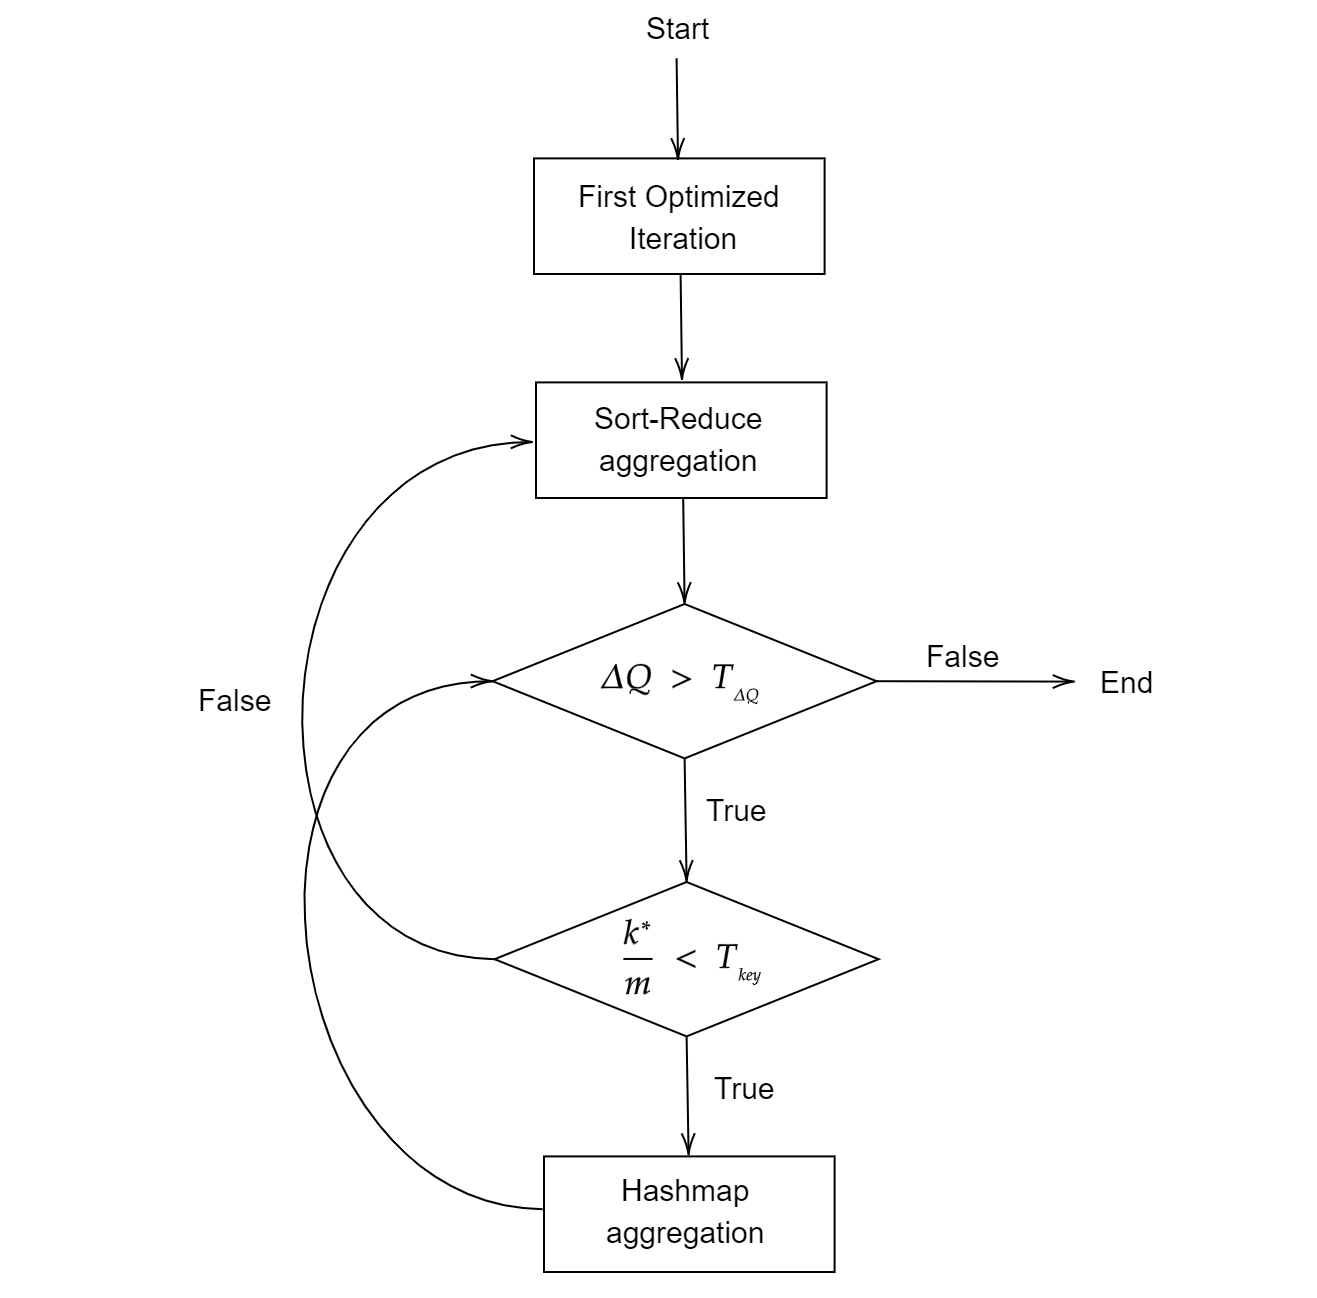
\includegraphics[width=0.7\linewidth]{0-resources/adaptive_schema}
	\caption{Schema of the Adaptive Optimization phase: before starting a new optimization routine, we check if the value $\frac{k^*}{m}$ falls below a given threshold: if it happen, we will use the hashmap based routine, otherwise we use the sort-reduce routine.}
	\label{fig:adaptiveschema}
\end{figure}
The Figure \ref{fig:adaptiveschema} shows a schematic diagram of the optimization phase logic. Now all it takes is to find the right values of $T_{key}$ that allow us to switch between the hashmap-based version when performs better. From the data presented in the next chapter, we observe that the two version take about the same time to perform an iteration of optimization when $\frac{k^*}{m}$ is between $0.3$ and $0.4$. When  $\frac{k^*}{m} > 0.4 $, the sort-reduce approach performs better; when  $\frac{k^*}{m} < 0.3 $, the hashmap approach performs better.
So we fixed the value of $T_{key}$ equals to $0.3$.\\
As regards the aggregation phase, we use the hashmap based approach in the adaptive algorithm, because, still from the observations presented in the previous chapter, we notice that this version tends to perform better with respect to the sort-version thanks to the reduction of the possible number of keys that we insert caused by the reduction of possible communities.
\subsection{Analysis}
\begin{table}[h]
	\centering
	\begin{tabular}{ |l||r||r|r|}
		\hline
		\multicolumn{4}{|c|}{Execution Times (in milliseconds) and Modularity} \\
		\hline
		Graph & Adaptive & PSR-Louvain & PH-Louvain \\
		\hline
		\multirow{ 2}{*}{coPapersDBLP}				& 369.14 	&  419.59  	&  412.79 \\
													& 0.8543 	&  0.8544  	&  0.8544 \\\hline
		\multirow{ 2}{*}{patentCite} 				& 1 660.79	& 1 796.88 	& 2 555.14 \\
													& 0.7927	& 0.7911   	& 0.7878 \\\hline
		\multirow{ 2}{*}{packing-500x100x100-b050}	& 993.35    & 1 045.25 	& 1 090.03 \\
													& 0.9403	& 0.9434 	& 0.9416 \\\hline
		\multirow{ 2}{*}{soc-pokec-relationship}	& 1 636.53	& 1 843.95 	& 2 186.81 \\ 
													& 0.6935 	& 0.6934 	& 0.6852 \\ \hline
		\multirow{ 2}{*}{delaunay\_n23 }			& 987.63 	& 1 020.23 	& 1 319.22 \\
													& 0.9856 	& 0.9856 	& 0.9857 \\\hline
		\multirow{ 2}{*}{soc-LiveJournal1}			& 2 078.29  & 2 187.45 	& 2 677.51 \\
													& 0.7493 	& 0.7491 	& 0.7482 \\\hline
		\multirow{ 2}{*}{wikipedia\_link\_ja} 		& 1 919.34  & 2 654.88 	& 2 305.11 \\
													& 0.5691	& 0.5690 	& 0.5724 \\\hline
		\multirow{ 2}{*}{hollywood-2009} 			& 1 685.98	& 2 092.09 	& 1 758.27 \\
													& 0.7542 	& 0.7542 	& 0.7542 \\\hline
		\multirow{ 2}{*}{wikipedia\_link\_it} 		& 2 417.01	& 3 875.04 	& 2 732.99 \\
													& 0.7190	& 0.7190 	& 0.7196 \\\hline
		\multirow{ 2}{*}{wikipedia\_link\_fr} 		& 2 741.07 	& 3 910.95 	& 3 273.91 \\
													& 0.6834	& 0.6834 	& 0.6871 \\\hline
		\multirow{ 2}{*}{com-orkut }				& 6 282.37	& 7 566.90 	& 7 484.10 \\
													& 0.6616	& 0.6613 	& 0.6629 \\\hline
		\multirow{ 2}{*}{wikipedia\_en(dbpedia)}	& 4 655.72	& 5 287.65 	& 6 464.03 \\
													& 0.6612 	& 0.6612 	& 0.6618 \\\hline
		\multirow{ 2}{*}{indochina-2004}			& 2 277.44 	& 2 899.50 	& 2 303.52 \\
													& 0.9632	& 0.9632 	& 0.9632 \\\hline
	\end{tabular}
	\caption{\label{tab:adaptive} Adaptive vs PSR-Louvain vs PH-Louvain}
\end{table} 
\newpage
\noindent In this section we analyze the results obtained by the Adaptive algorithm: we make a comparison between this version and the two other version presented previously in this thesis; besides we make a comparison with two interesting library: Nvidia's cuGraph and Gunrock.
To make our test we use the same 13 datasets presented in Chapter \ref{Dataset} and the same Ubuntu 18.04.4 LTS machine used in the test presented previously. We remind that the machine is equipped with a 2.10GHz Intel(R) Xeon(R) Silver 4110 CPU, a TITAN Xp GPU with 12 GB of memory and CUDA 10.2.
\begin{figure}[t!]
	\centering
	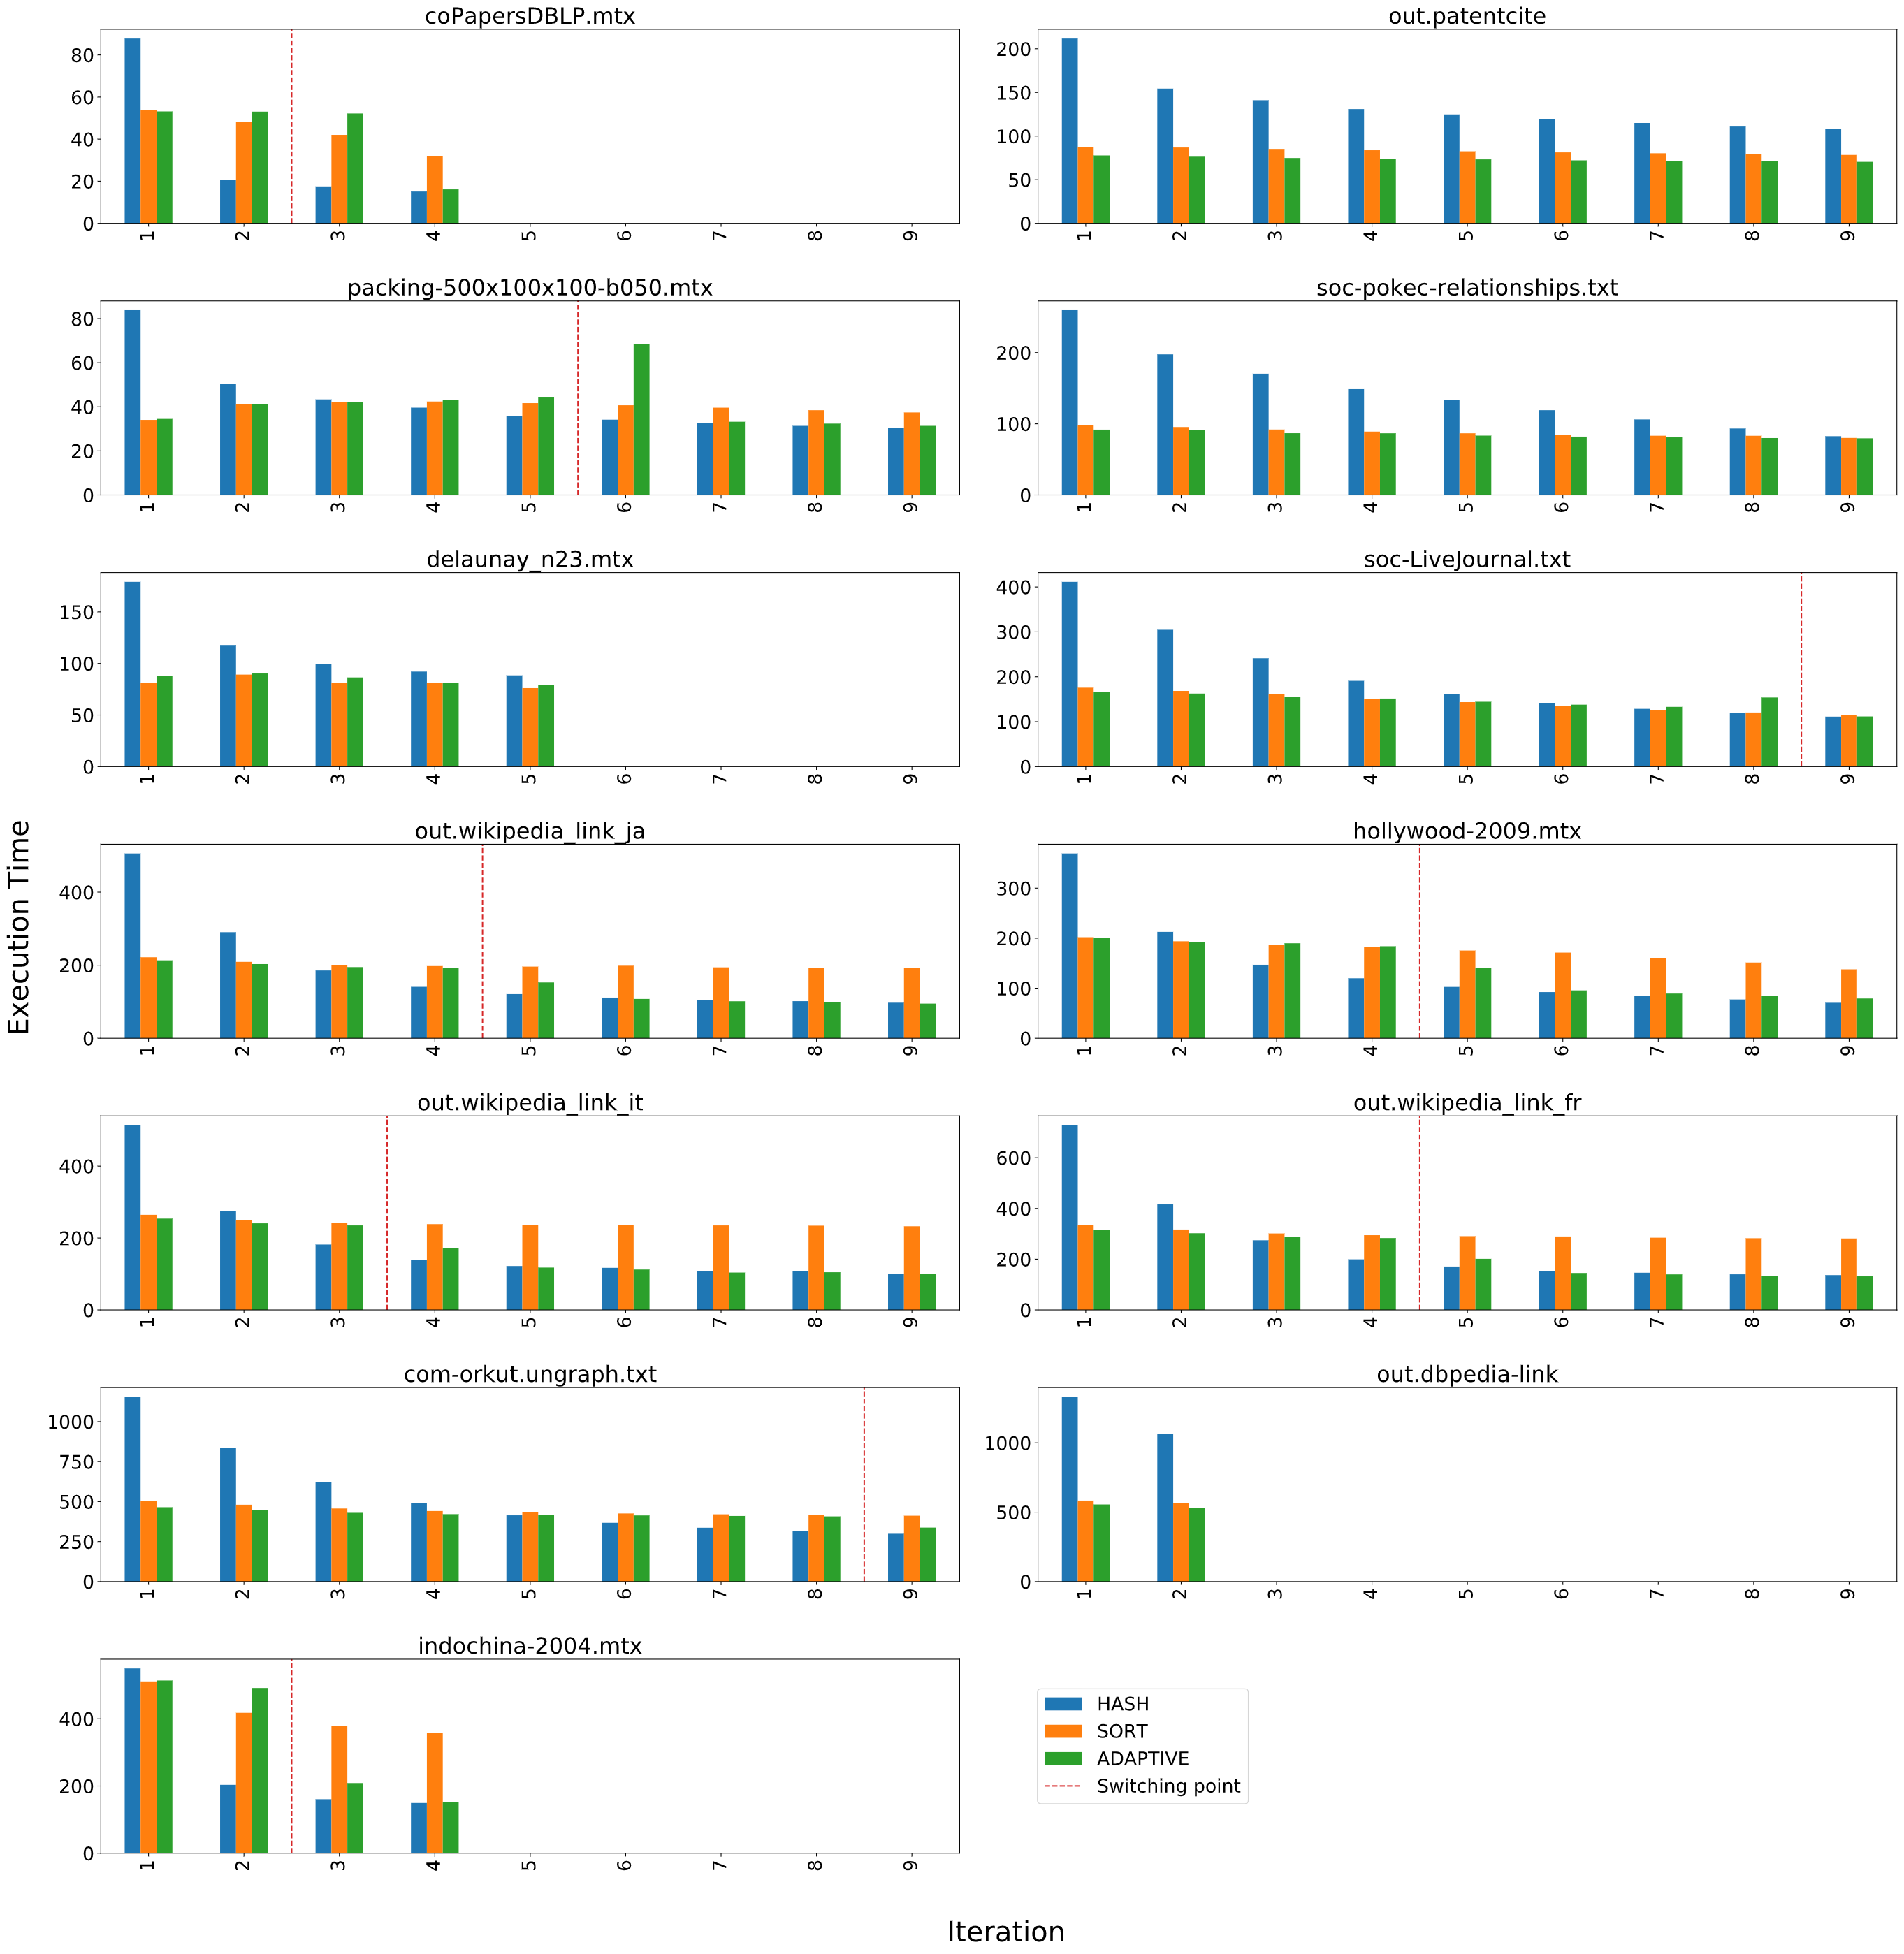
\includegraphics[width=1\linewidth]{0-resources/adaptive-vs-other}
	\caption{Execution time in the first ten iteration of the first optimization phase, excluding the first optimized iteration. The dotted red line indicate that, from the next iteration, the Adaptive algorithm uses a Hashmap based approach. Before the line the algorithm uses a Sort-Reduce approach.}
	\label{fig:adaptive-vs-other}
\end{figure}
We start comparing and analyzing our adaptive respect to PSR-Louvain and the PH-Louvain presented in Chapter \ref{GPUalg}. We present the results in terms of time and in terms of modularity in the Table \ref{tab:adaptive}. We use a threshold $T_{\Delta Q}$ equals to 0.01. As we can see, we have an improvement in terms of times without any loss in terms of modularity: this is thanks to correctness of the params $T_{key}$ that allow us to switch between the two approaches when it's needed. 
We study in detail the behaviour of the algorithm: Figure \ref{fig:adaptive-vs-other} shows the execution time of the first ten iteration of the first optimization phase for the PH-Louvain (in blue), the PSR-Louvain version (in Orange) and the Adaptive version (in green). The red dotted vertical line highlight when the Adaptive algorithm switch behaviour from the sort-reduce one to the hashmap one. When the algorithm switch from the first approach to the second one, the algorithm doesn't choose the first one until the next phase. We notice that in the dataset in which the sort-reduce version performs better (for example in the dataset wikipedia\_en (dbpedia)) the algorithm use only this version and doesn't perform any change. In the other cases, we notice that the first iteration with the hashmap aggregator of the Adaptive algorithm show a little delay with respect to the same iteration of the PH algorithm: this is due to the deallocation of the support variable used in the sort-reduce approach and the allocation of the hashmap variables, as in the second iteration of the PH-Louvain, after the first optimized phase (Chapter \ref{alg-comp}). Besides, we investigate the behaviour of the algorithm also in the other optimization phase, in order to explain why the Adaptive version performs better than the other two approaches also in the dataset in which the PH-Louvain performs better in the first iteration phase, as indochina-2004. We notice that the algorithm uses the sort-reduce approach in the phases subsequent to after the first for the most part of the iterations: this caused the increment of the performances because, as we present in the Chapter \ref{alg-comp},  the sort-reduce approach tend to perform better in the first iterations of the phases, and these phases tends to execute less iteration.\\
Now we present a comparison between our algorithm and other two version of the Louvain Algorithm for the GPU: the first one is part of the Nvidia's RAPIDS cuGraph library,  a collection of GPU accelerated graph algorithms, actually still under development but aviable in  with a open-source license on GitHub; the second one is part of the Gunrock library, a CUDA  library for graph-processing designed specifically for the GPU released in June 2019. The Gunrock team is one of the main contributors of the cuGraph library and some modules of the first library is integrated in the second. Both the algorithm doesn't implement any pruning approach or any adaptive approach.

In the optimization phase, the first algorithm use an hashmap for each node to aggregate the tuple (node, community, weight): each map is assigned to a unique vertex and the algorithm insert the weight using only the 
community as key. If there is already an entry in the map, the map automatically sum up the values. After this, the algorithm calculate the delta for each entry of the map and than select the maximum. To implement the hashmaps, they use two vector of lenght $m$, where $m$ is the number of nodes, and assign to each node a private part of them in which insert its keys and values. They assign to each vector a space of size equals to the size of its neighbourhood and use an open-addressing procedure for the conflict, checking the subsequent free position. 
After this, they use a procedure similar to the Select Max sub-phase of the Prune-Sort-Reduce algorithm: 
they use the method \verb|thrust::reduce_by_key| to get the best values using the two vector as values and as a keys a vector that keep track to which source node is assigned each position in the hashmap vectors. Besides, this algorithm propose a different techniques to avoid simultaneous swap: instead of forcing the node in single communities to select a community with a greater id like us, they permit to the nodes to select a community with a greater id only in the even iteration and to select a community with a lower id only in the odd iteration. \\
To contract the graph, this algorithm use a procedure similar to the one proposed in the Prune-Sort-Reduce algorithm: first they renumber the communities, then they create a vector of (community source, community destination, weights) from the edges vector replacing each node with the relative communities, and finally they sort and reduce this vector.

The Gunrock algorithm use a logic similar to the our Prune-Sort-Reduce version to aggregate the nodes:they copy the edges changing the destination node with the corresponding community, than they sort all key-value pairs, and they use segmented reduce to accumulate the values in the continuous segments. Finally the algorithm use a reduction by keys to select the maximum value. To aggregate the graph, they use a procedure similar to cuGraph and our Prune-Sort-Reduce version. Our study to this algorithm find an error in the stopping criteria logic of the optimization phase: this algorithm, to calculate the difference $\Delta Q$ between two 
configuration, sum all the various $\Delta Q_{i \rightarrow c_z^*}$ for each node $i$ that change its community to $c_z^*$ obtained during the optimization phase to the previous modularity value. This values is incorrect because, changing all the communities simultaneously, the various $l$ and $k_c$ values of the equation \ref{delta_q} are referred to a situation that isn't the actual any more. This causes a wrong calculation of the temporary modularity score, that can also exceed its upper bound of one during this phase. This causes also a reduction in the execution time because this algorithm doesn't recalculate the modularity after each iteration.
Nevertheless, our tests on this library highlight that the algorithm doesn't iterate the optimization phase more than 10 times: this early stop criteria, combined with a recalculation of the final score after the optimization, allows the algorithm to find a valid configuration.\\
To setup our test in order to have comparable results between these three versions, we set the threshold $T_{\Delta Q}$ equals to 0.01 for the Adaptive and cuGraph version. To set this value we change the source code of the library because this value is fixed in the actual release. Using this parameters, the execution time and the final modularity are comparable with the Gunrock version. 
\begin{table}[t!]
	\centering
	\begin{tabular}{ |l||r||r|r|}
		\hline
		\multicolumn{4}{|c|}{Execution Times (in milliseconds) and Modularity} \\
		\hline
		Graph & Adaptive & cuGraph & Gunrock \\
		\hline
		\multirow{ 2}{*}{coPapersDBLP}				& 369.14 	&  589.27  	&  561.15 \\
													& 0.8543 	&  0.8541  	&  0.8416 \\\hline
		\multirow{ 2}{*}{patentCite} 				& 1 660.79	& 1 175.62 	&  1 615.13 \\
													& 0.7927	& 0.7936   	&  0.7806 \\\hline
		\multirow{ 2}{*}{packing-500x100x100-b050}	& 993.35    & 885.77	&  734.37 \\
													& 0.9403	& 0.9437 	&  0.9372\\\hline
		\multirow{ 2}{*}{soc-pokec-relationship}	& 1 636.53	& 1 546.91 	& 1 019.44 \\ 
													& 0.6935 	& 0.7109 	& 0.6935 \\ \hline
		\multirow{ 2}{*}{delaunay\_n23 }			& 987.63 	& 1 041.23 	& 1 608.63 \\
													& 0.9856 	& 0.9877 	& 0.9860 \\\hline
		\multirow{ 2}{*}{soc-LiveJournal1}			& 2 078.29  & 2 474.60 	& 2 226.35 \\
													& 0.7493 	& 0.7504 	& 0.7504 \\\hline
		\multirow{ 2}{*}{wikipedia\_link\_ja} 		& 1 919.34  & 2 744.37 	& 2 283.09 \\
													& 0.5691	& 0.5825 	& 0.5647 \\\hline
		\multirow{ 2}{*}{hollywood-2009} 			& 1 685.98	& 2 210.50 	& 2 028.64 \\
													& 0.7542 	& 0.7511 	& 0.7468 \\\hline
		\multirow{ 2}{*}{wikipedia\_link\_it} 		& 2 417.01	& 4 184.10 	& 2 653.13 \\
													& 0.7190	& 0.7326 	& 0.7112 \\\hline
		\multirow{ 2}{*}{wikipedia\_link\_fr} 		& 2 741.07 	& 4 017.74	& 3 392.85 \\
													& 0.6834	& 0.6848	& 0.6759  \\\hline
		\multirow{ 2}{*}{com-orkut }				& 6 282.37	& -		 	& - \\
													& 0.6616	& - 		& - \\\hline
		\multirow{ 2}{*}{wikipedia\_en(dbpedia)}	& 4 655.72	& -			& - \\
													& 0.6612 	& - 		& - \\\hline
		\multirow{ 2}{*}{indochina-2004}			& 2 277.44 	& - 		& - \\
													& 0.9632	& - 		& - \\\hline
	\end{tabular}
	\caption{\label{tab:ad-cu-gun} Adaptive vs cuGraph vs Gunrock}
\end{table} 
We present the results in the Table \ref{tab:ad-cu-gun}. The first thing that we notice is that our algorithm is better optimized in terms of memory: on our machine we can analyze graphs up to $\sim 175 000 000$ edges, instead our competitor go out of memory when the graph has $\sim 90 000 000$. One of the reasons that allow us to reach graph of bigger size is the memory optimization of the our optimization phase: therefore, we divide the edges in some buckets of fixed size, we execute the phase, store the results and start the execution on another bucket; when all buckets are processed we update the communities. With this technique we reduce the amount of memory used to store the data in that phase from about $2m$, where $m$ is the number of edges of the graph, to $2 * s + n$, where $s$ is the bucket size and $n$ is the number of nodes (Chapter \ref{impl-details}). Besides, our test highlight that we use fewer memory to store the graph in the device memory. \\
In terms of modularity we notice that our algorithm is on pair with the cuGraph version that, for the reason presented previously, is more accurate than the Gunrock algorithm. In terms of performance we notice that our algorithm perform better to the bigger graphs. Analyzing the cuGraph optimization phase, we notice that this version tend to perform more iteration with respect to the Adaptive version: this behaviour is probably caused by the fact that they allow each node to select a community with a greater id or a smaller id intermittently.
We also notice that their optimization iteration tends to go faster iteration by iteration, acting as our Hashmap algorithm (Chapter \ref{hashmap-analysis}); furthermore, the optimization phase are generally slightly faster with respect to our hashmap approaches at the same iteration, and so this algorithm is quicker than ours when both performs the same number of iterations. It's not clear if the improvement is made by internal optimization of the operation or thanks to the fact that they uses an hashmap for each node instead of a global one: the analysis of this is left as future work. Finally we notice that the our algorithm contract the graph quickly by the using the hashmap approach instead of the sorting one (Chapter \ref{alg-comp}).


Analyzing the Gunrock algorithm, we notice this algorithm does not calculating the modularity after each step and it hav an early stop at the tenth iteration: this causes a gain in term of time with respect of our algorithm if we execute more than ten iteration without swapping behaviour to hash-mode (or when the gain that we have using map is not high) , thanks to the time saved from the modularity calculation. On the other hand, they doesn't stop the iteration when they should: this can lead to perform extra useless iteration of the optimization phase. In the wrong case, this behaviour can also to a decrease of global modularity between two iteration and therefore to doesn't find the local maximum. Surprisingly, this algorithm find however a good modularity score. We left as future work the analysis of this behaviour, and if we can avoid to perform the modularity calculation at each iteration to reduce the execution time without significant loss in modularity. 


Concluding, our adaptive algorithm performs very well even compared to a some Louvain algorithm presented in some library related with Nvidia: we even occupy fewer memory and we perform better on the largest graphs.\\ The pruning approach helps the algorithm to reduce time, but it highly depends on the graphs. This approach can be very useful in multi-gpu algorithms, where one of the bottleneck is the data transfer between the global memory to the GPU, even using the an hashmap to aggregate, that our tests show that have a smaller improvement with respect to the sort-reduce aggregation technique. This technique can be useful also to compute the modularity on graph that doesn't fit in the device memory. We left the design and the analysis of that algorithm as a future work. \\
The adaptive behaviour is very effective and allow us to reduce the computation time of the first inefficient operation with the hashmap. We left as future work the analysis of the performance of using a private hashmap for each node instead a global one, and the impact using this behaviour on a adaptive approach.
